\subsection{Mono-jet channel}

\begin{figure}[t]
  \centering
    \begin{subfigure}[t]{0.495\textwidth}
      \centering
      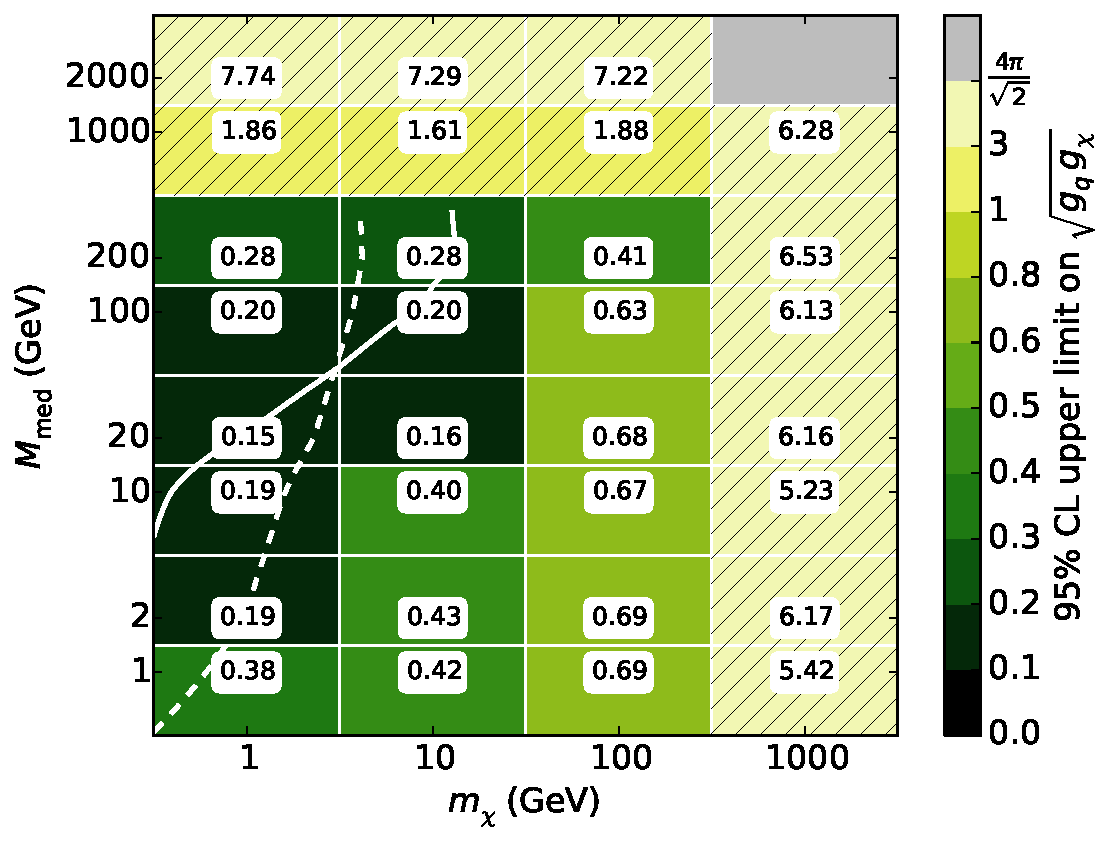
\includegraphics[width=1.\textwidth]{figures/grid_basepoints_SVD_rat05_monojet.pdf}
      \caption{}
    \end{subfigure}
    \begin{subfigure}[t]{0.495\textwidth}
      \centering
      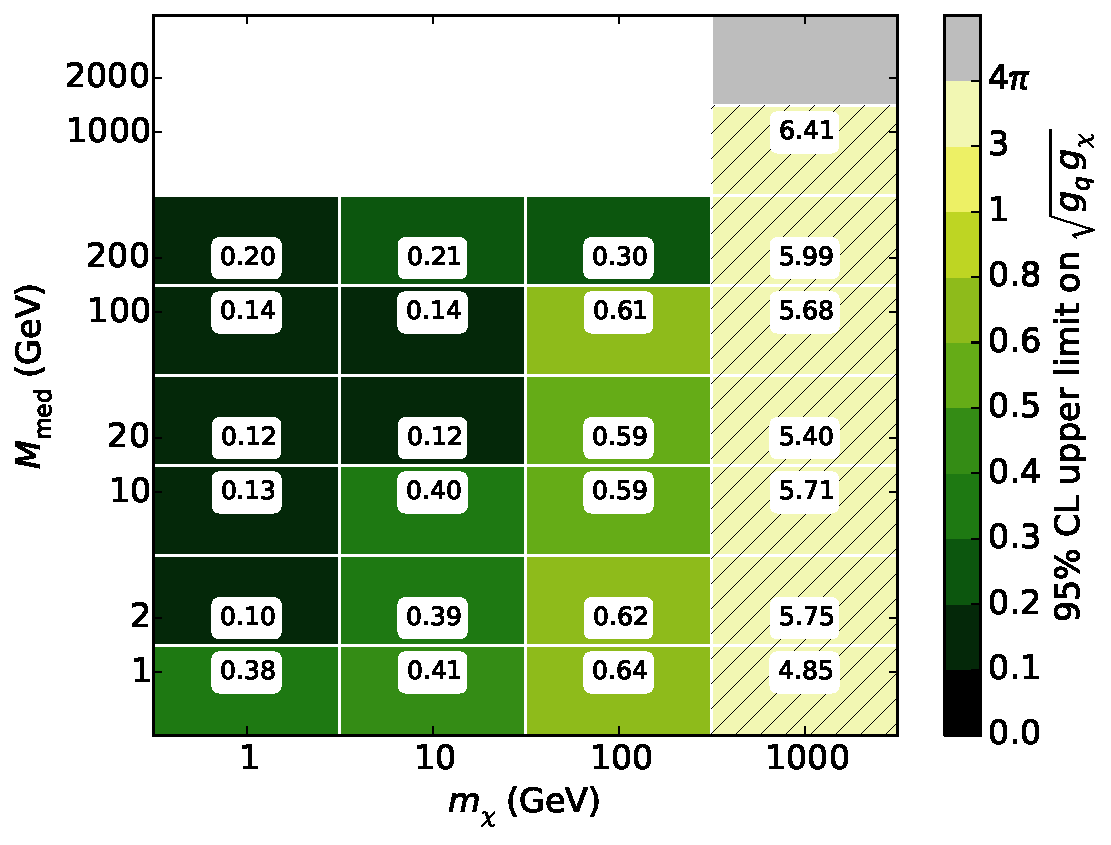
\includegraphics[width=1.\textwidth]{figures/grid_basepoints_SVD_rat1_monojet.pdf}
      \caption{}
    \end{subfigure}
    \begin{subfigure}[t]{0.495\textwidth}
      \centering
      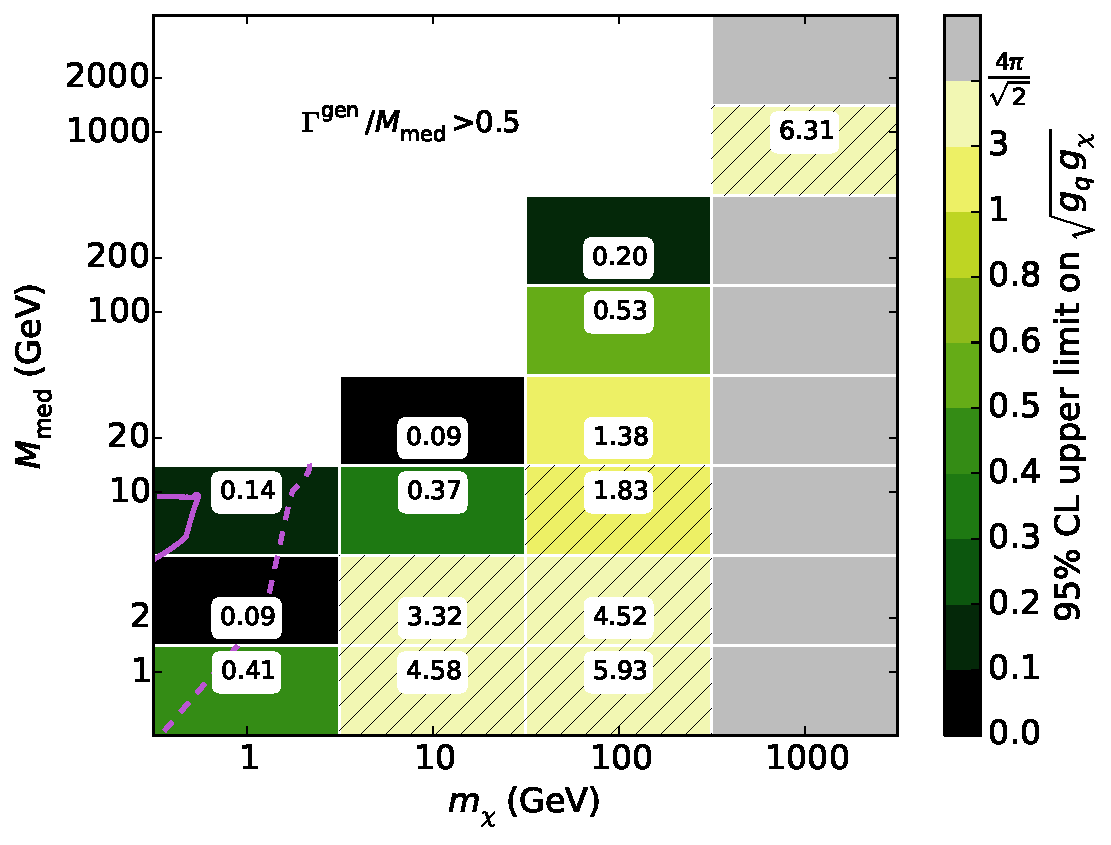
\includegraphics[width=1.\textwidth]{figures/grid_basepoints_SVD_rat2_monojet.pdf}
      \caption{}
    \end{subfigure}
    \begin{subfigure}[t]{0.495\textwidth}
      \centering
      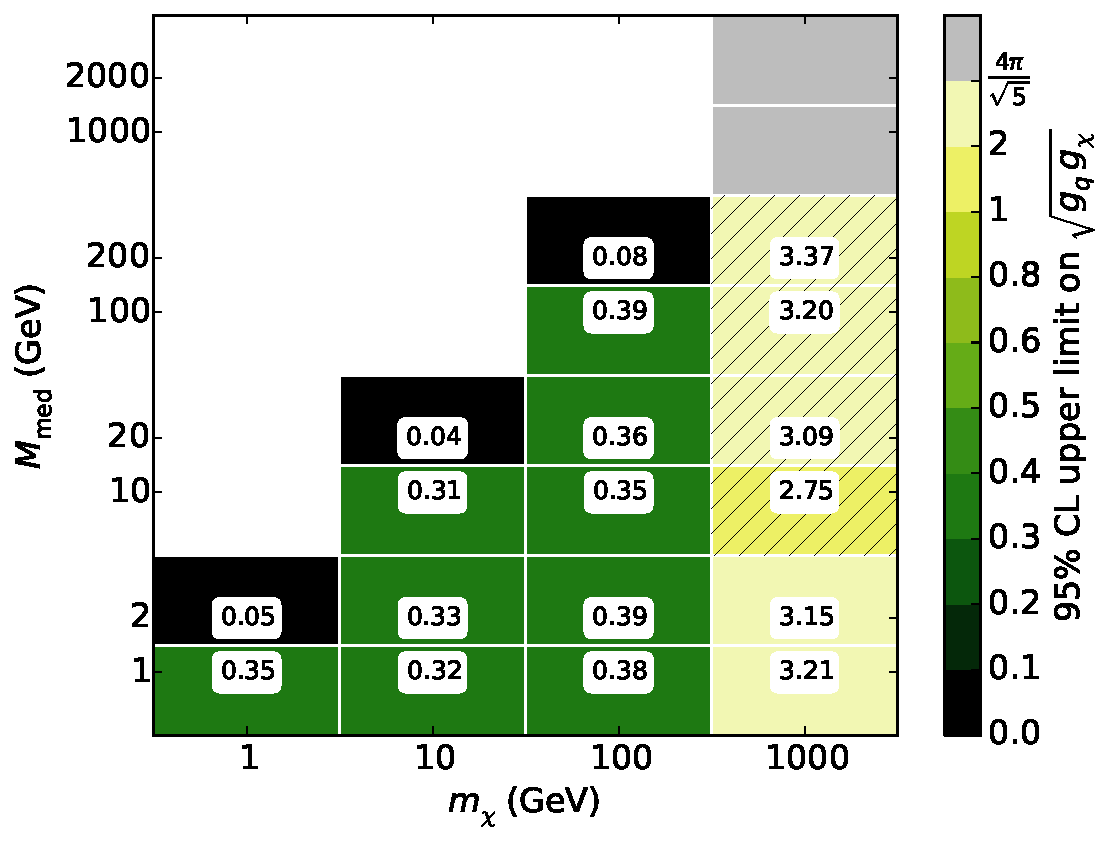
\includegraphics[width=1.\textwidth]{figures/grid_basepoints_SVD_rat5_monojet.pdf}
      \caption{}
    \end{subfigure}
    \caption{Upper limits on the coupling for the sV model, in the \monojet channel, for $\gX / \gq$ = 0.5 (a), 1 (b), 2 (c) and 5 (d). The grey region represents the phase space where no meaningful limit was obtained. The hatched region represents a limit which leads to a width greater than $\Mmed / 2$, so the validity of the calculation begins to fail.}
    \label{fig:Monojet_SVD_couplinglimit}
\end{figure}

\begin{figure}[h]
  \centering
    \begin{subfigure}[t]{0.495\textwidth}
      \centering
      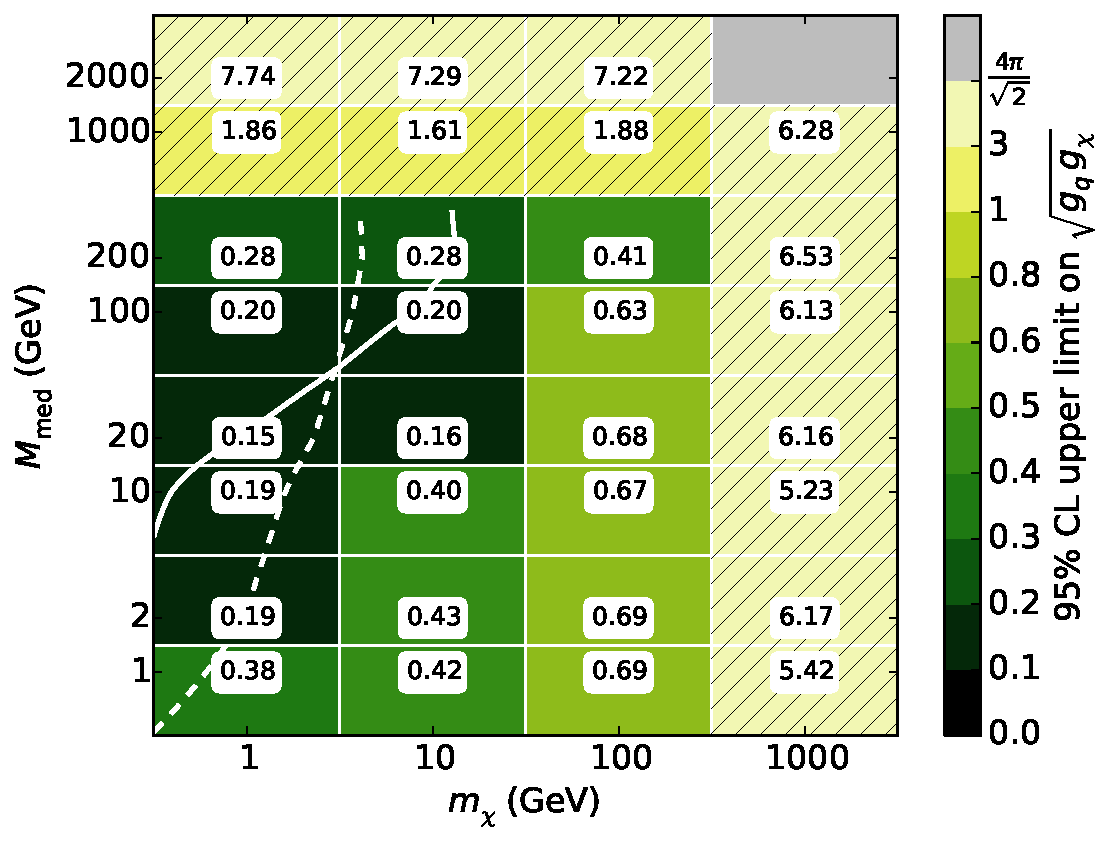
\includegraphics[width=1.\textwidth]{figures/grid_basepoints_SVD_rat05_monojet.pdf}
      \caption{}
    \end{subfigure}
    \begin{subfigure}[t]{0.495\textwidth}
      \centering
      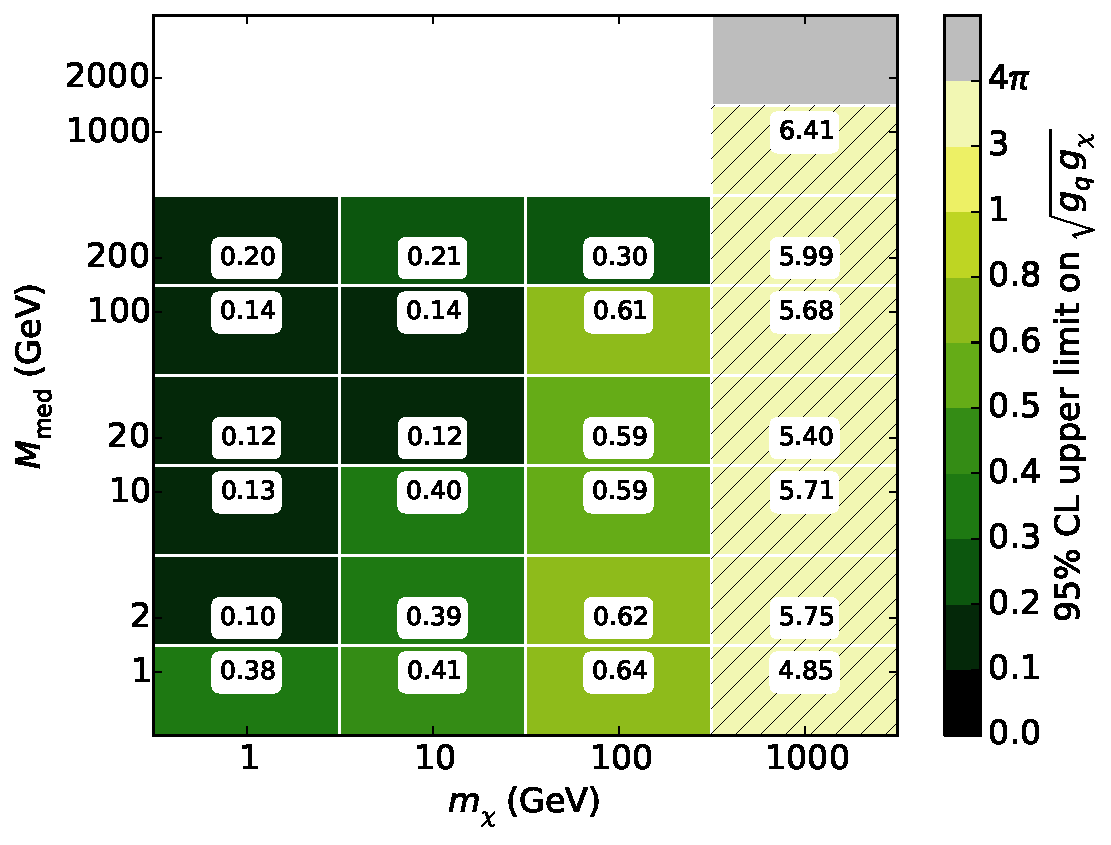
\includegraphics[width=1.\textwidth]{figures/grid_basepoints_SVD_rat1_monojet.pdf}
      \caption{}
    \end{subfigure}
    \begin{subfigure}[t]{0.495\textwidth}
      \centering
      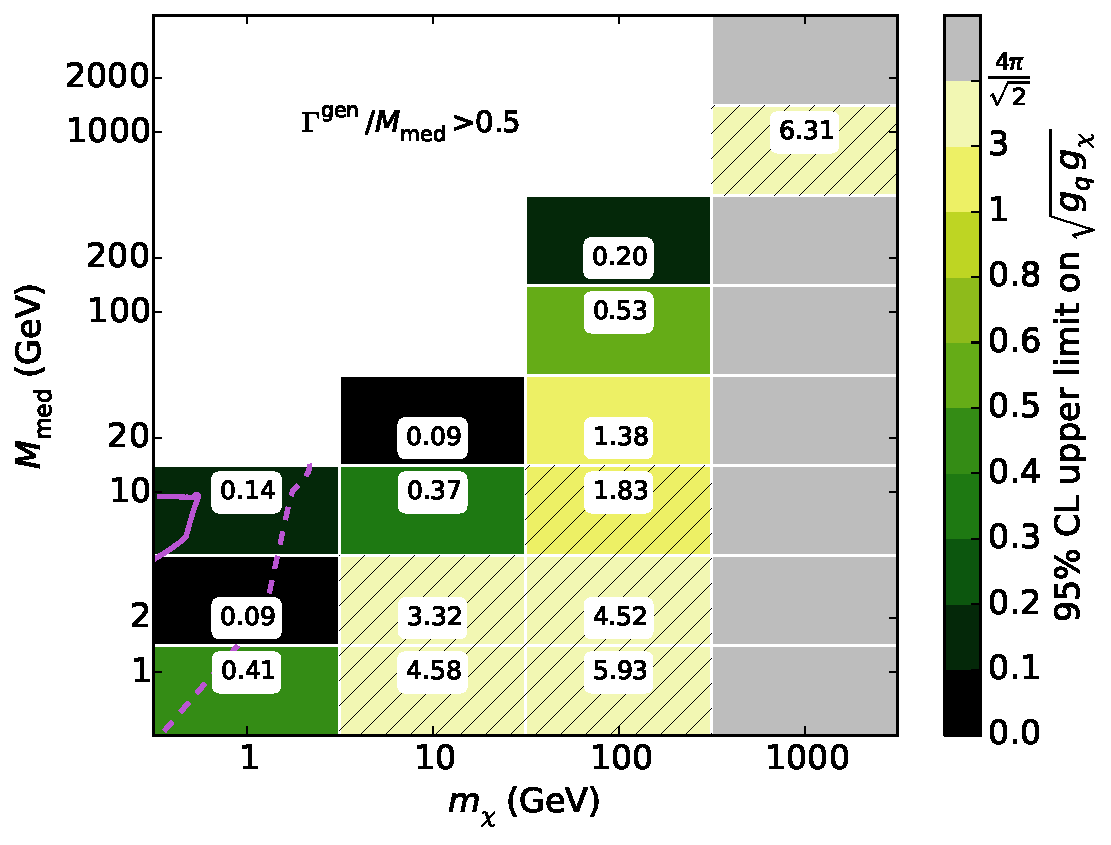
\includegraphics[width=1.\textwidth]{figures/grid_basepoints_SVD_rat2_monojet.pdf}
      \caption{}
    \end{subfigure}
    \begin{subfigure}[t]{0.495\textwidth}
      \centering
      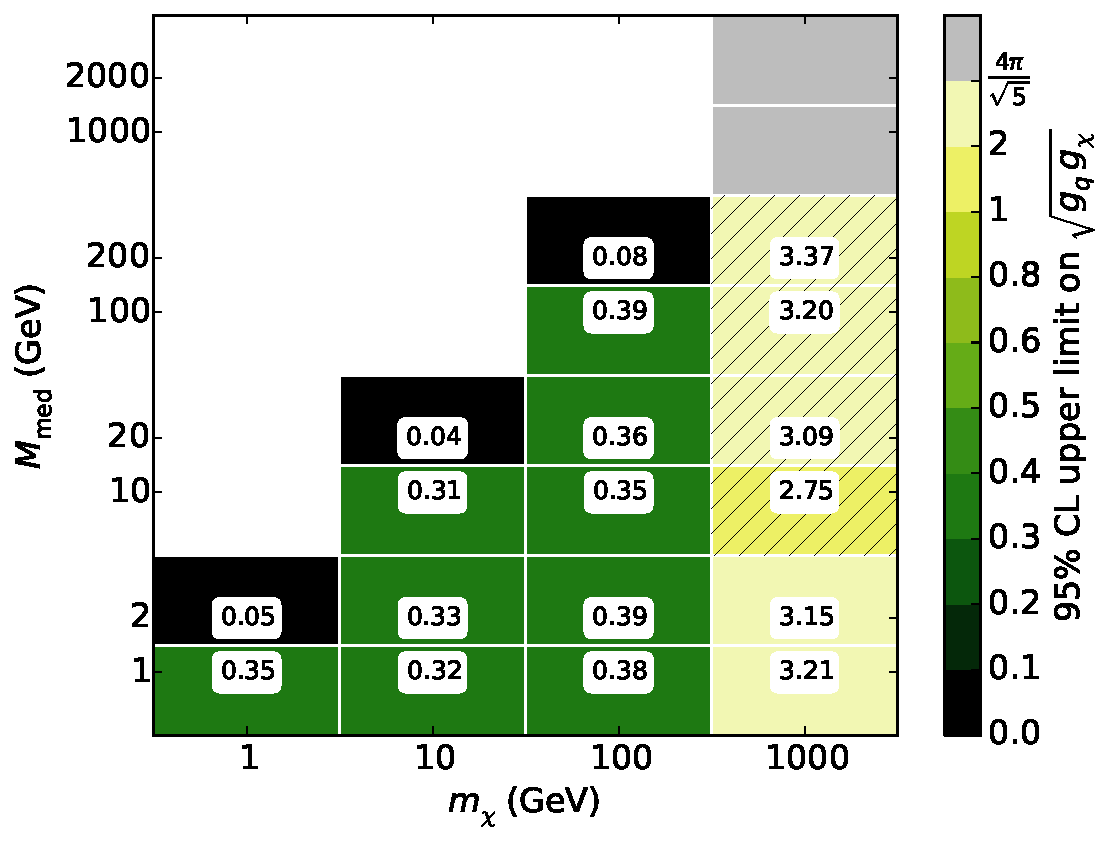
\includegraphics[width=1.\textwidth]{figures/grid_basepoints_SVD_rat5_monojet.pdf}
      \caption{}
    \end{subfigure}
    \caption{Upper limits on the coupling for the sA model, in the \monojet channel, for $\gX / \gq$ = 0.5 (a), 1 (b), 2 (c) and 5 (d). The grey region represents the phase space where no meaningful limit was obtained. The hatched region represents a limit which leads to a width greater than $\Mmed / 2$, so the validity of the calculation begins to fail. TO BE UPDATED WITH sA PLOTS.}
    \label{fig:Monojet_SVD_couplinglimit}
\end{figure}

Results discussion here.

\subsection{Mono-$Z$ channel}

\begin{figure}[h]
  \centering
    \begin{subfigure}[t]{0.495\textwidth}
      \centering
      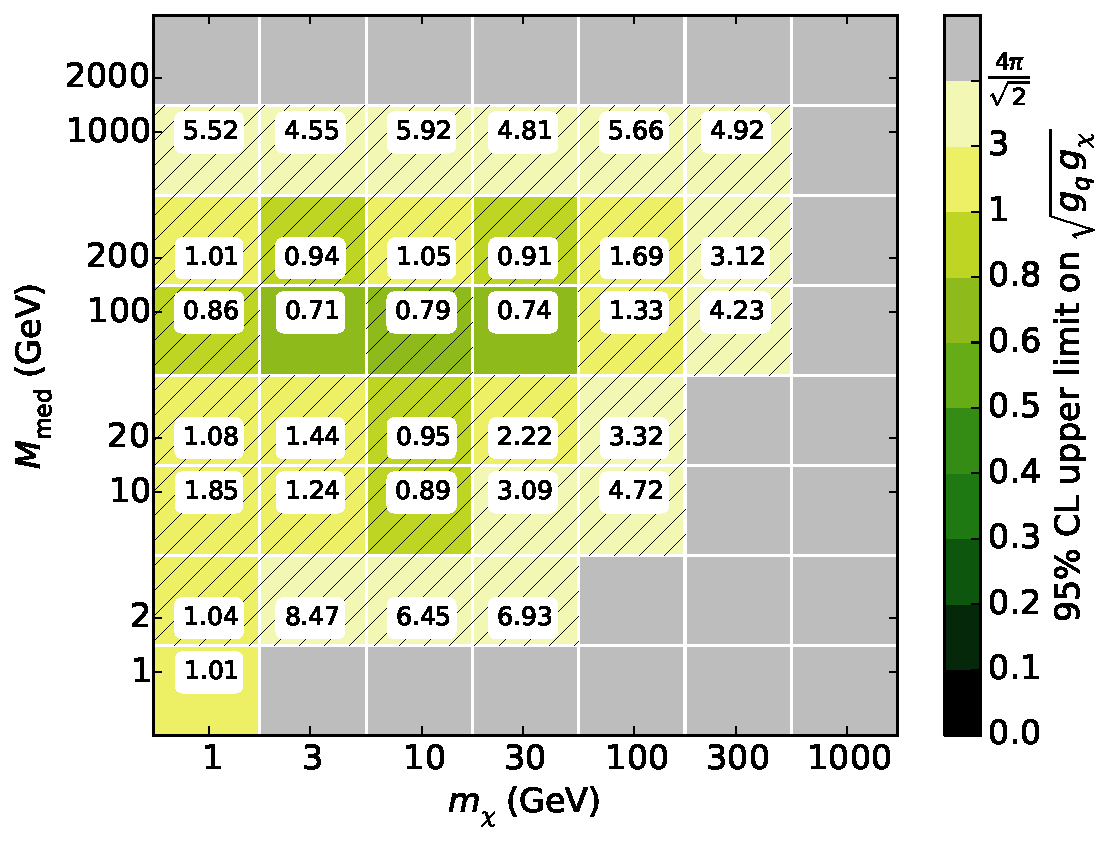
\includegraphics[width=1.\textwidth]{figures/grid_allpoints_SVD_rat05.pdf}
      \caption{}
    \end{subfigure}
    \begin{subfigure}[t]{0.495\textwidth}
      \centering
      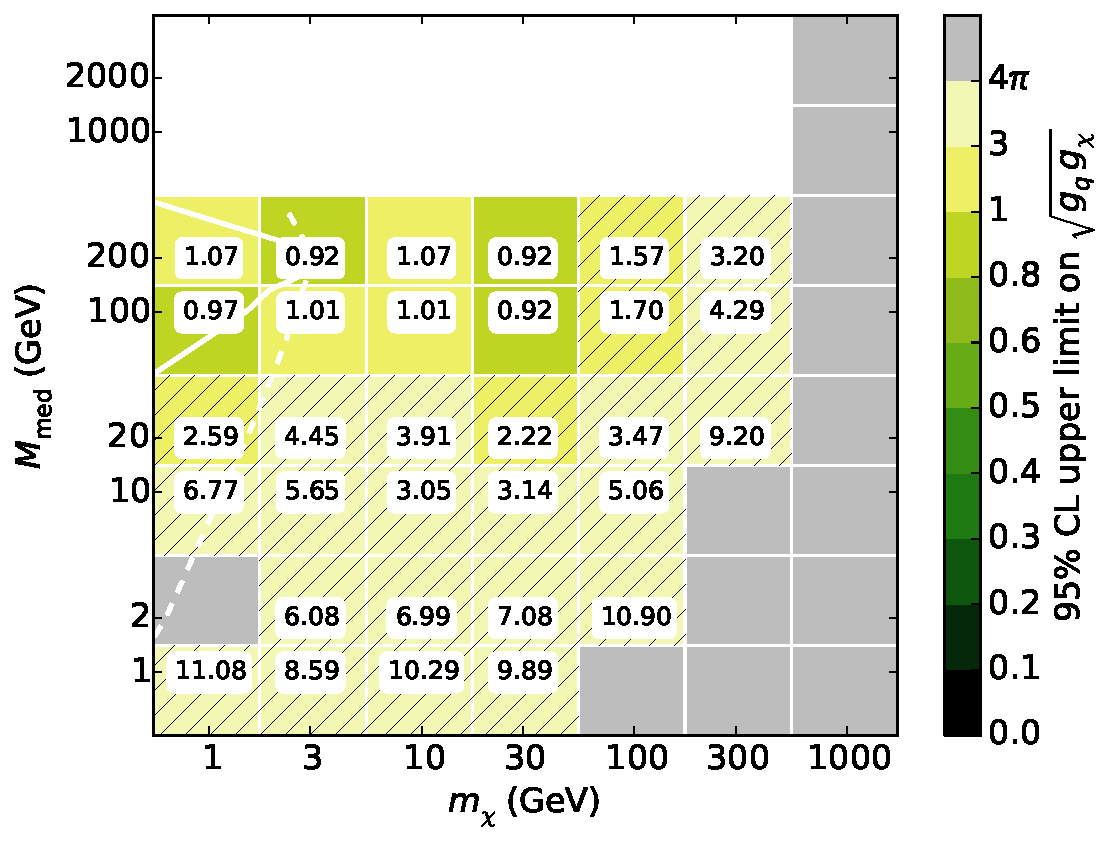
\includegraphics[width=1.\textwidth]{figures/grid_allpoints_SVD_rat1.pdf}
      \caption{}
    \end{subfigure}
    \begin{subfigure}[t]{0.495\textwidth}
      \centering
      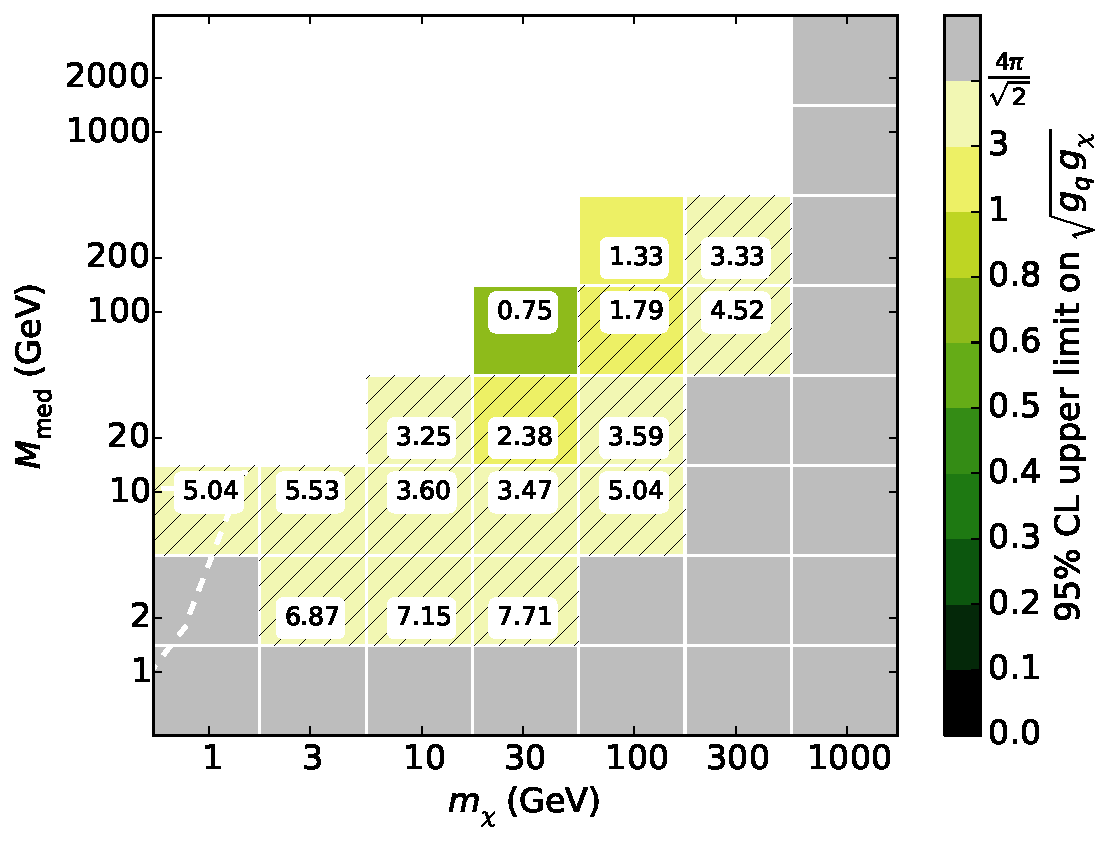
\includegraphics[width=1.\textwidth]{figures/grid_allpoints_SVD_rat2.pdf}
      \caption{}
    \end{subfigure}
    \begin{subfigure}[t]{0.495\textwidth}
      \centering
      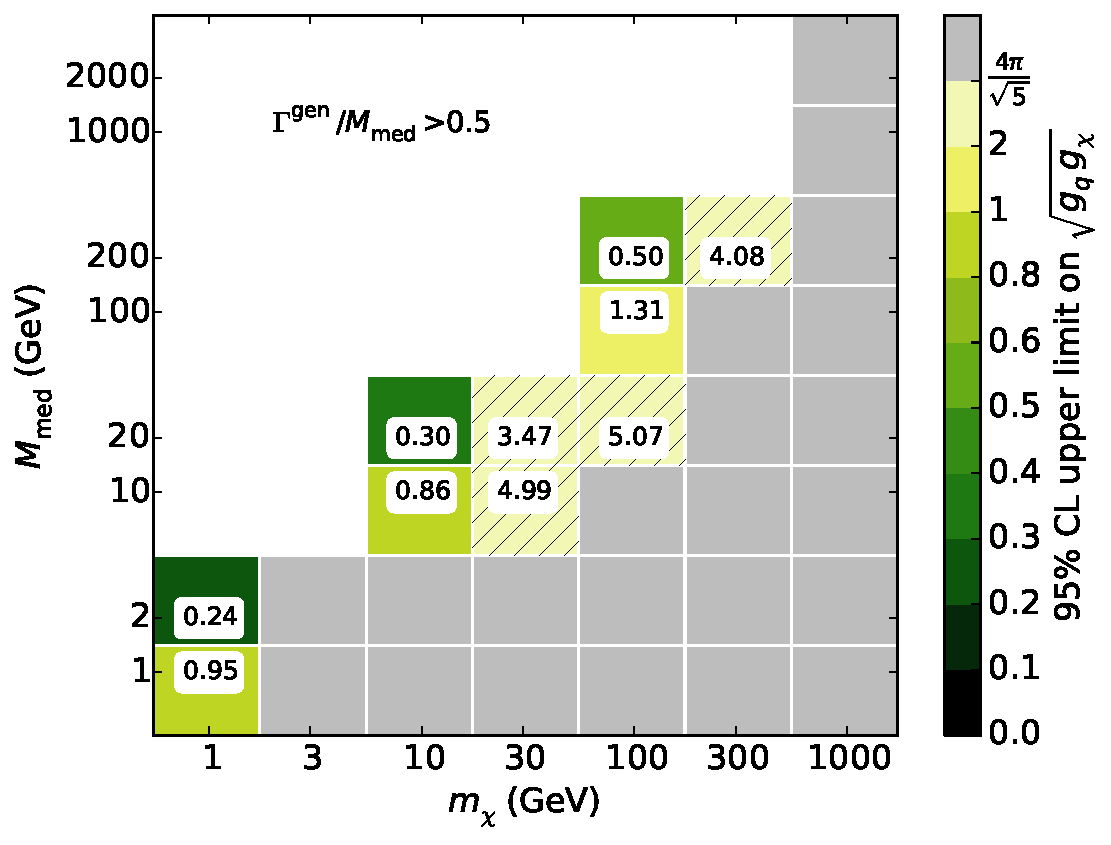
\includegraphics[width=1.\textwidth]{figures/grid_allpoints_SVD_rat5.pdf}
      \caption{}
    \end{subfigure}
    \caption{Upper limits on the coupling for the sV model, in the \monoZ channel, for $\gX / \gq$ = 0.5 (a), 1 (b), 2 (c) and 5 (d). The grey region represents the phase space where no meaningful limit was obtained. The hatched region represents a limit which leads to a width greater than $\Mmed / 2$, so the validity of the calculation begins to fail.}
    \label{fig:MonoZ_SVD_couplinglimit}
\end{figure}

\begin{figure}[h]
  \centering
    \begin{subfigure}[t]{0.495\textwidth}
      \centering
      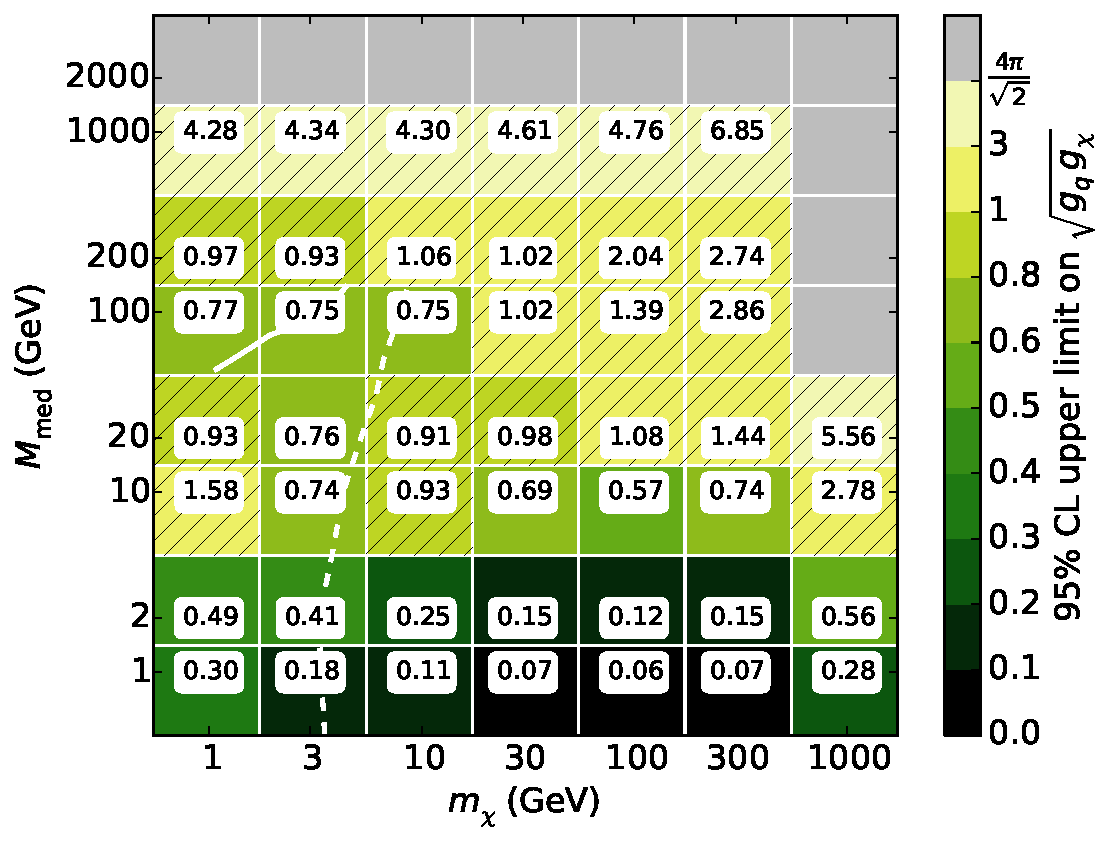
\includegraphics[width=1.\textwidth]{figures/grid_allpoints_SAD_rat05.pdf}
      \caption{}
    \end{subfigure}
    \begin{subfigure}[t]{0.495\textwidth}
      \centering
      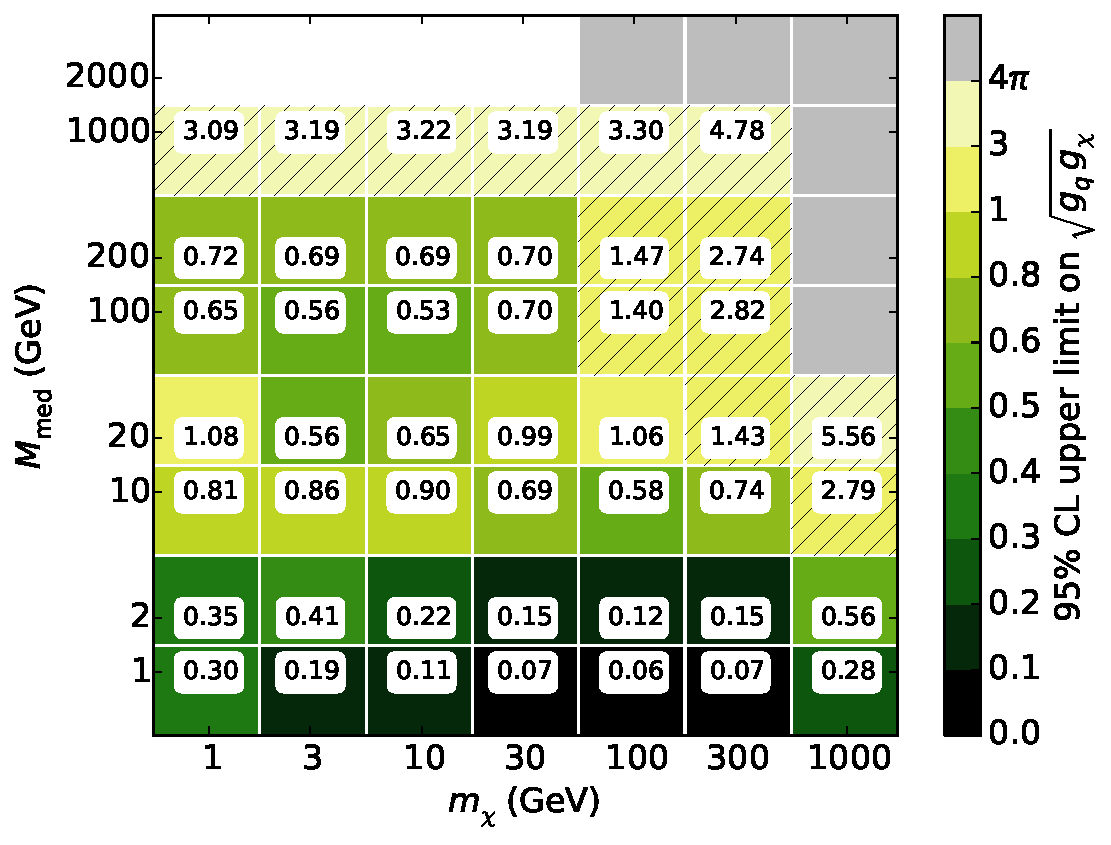
\includegraphics[width=1.\textwidth]{figures/grid_allpoints_SAD_rat1.pdf}
      \caption{}
    \end{subfigure}
    \begin{subfigure}[t]{0.495\textwidth}
      \centering
      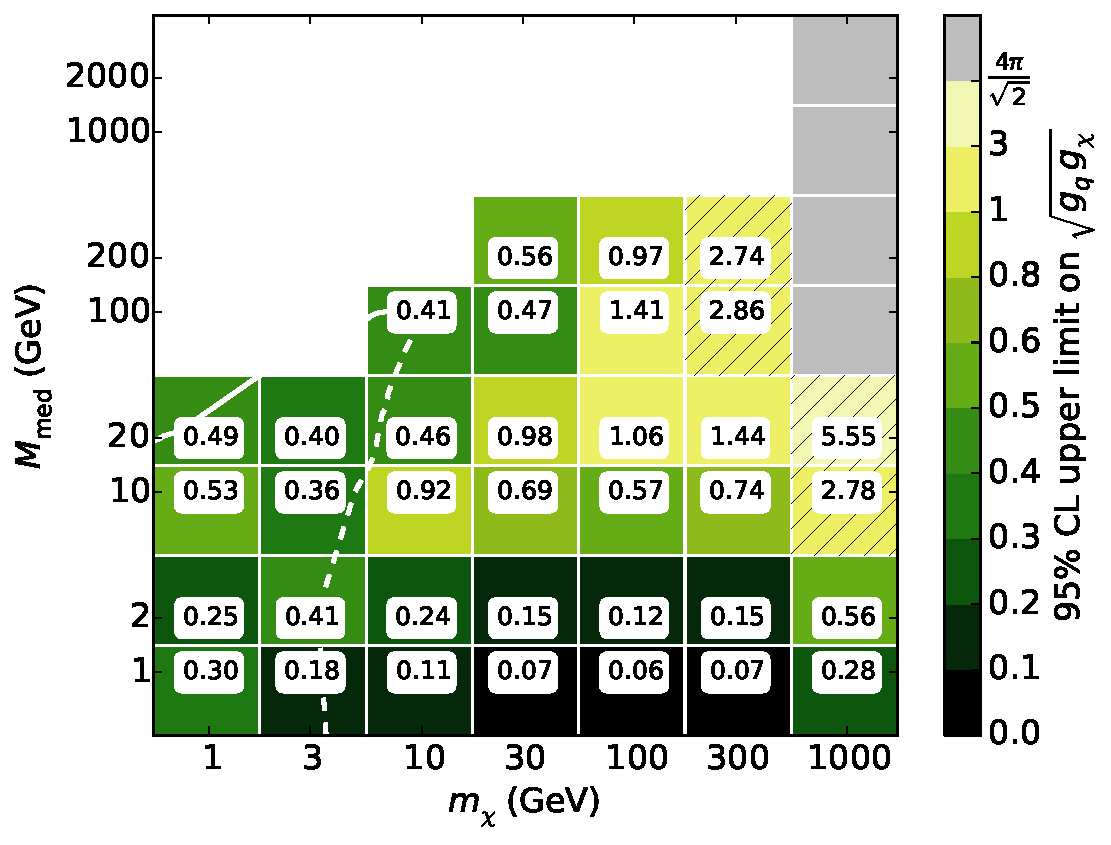
\includegraphics[width=1.\textwidth]{figures/grid_allpoints_SAD_rat2.pdf}
      \caption{}
    \end{subfigure}
    \begin{subfigure}[t]{0.495\textwidth}
      \centering
      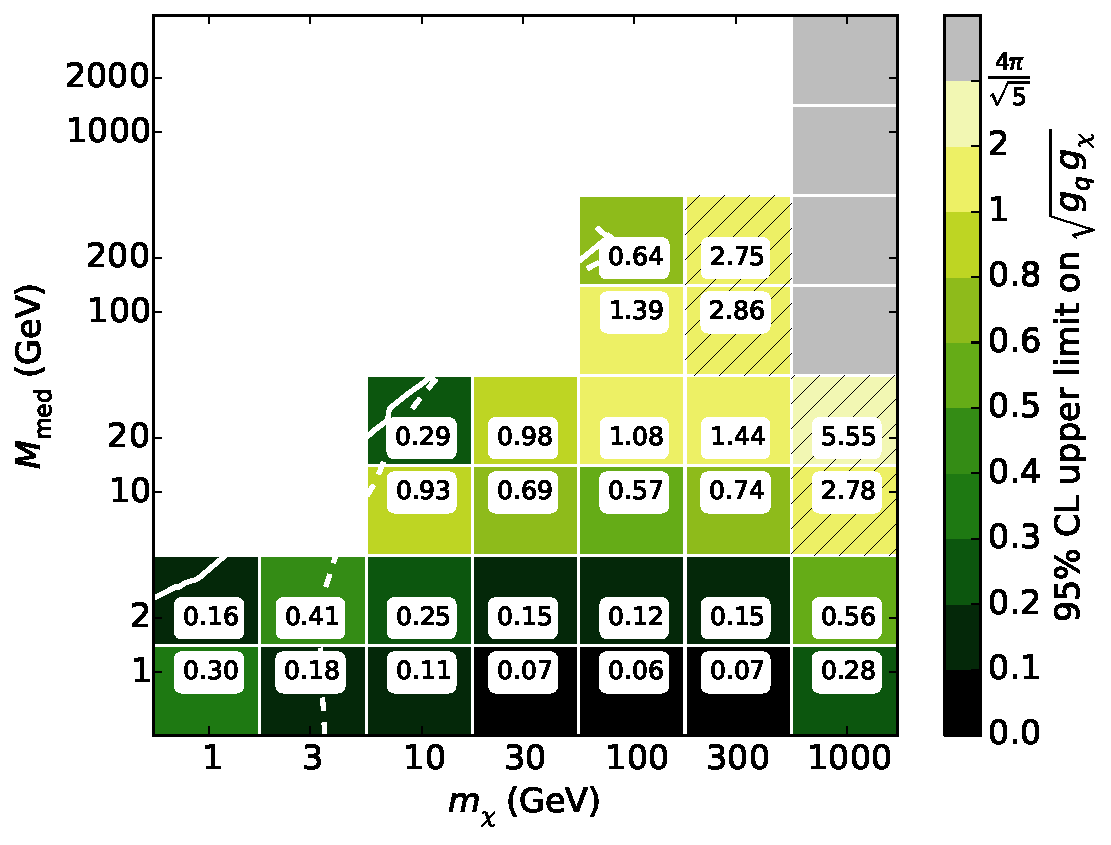
\includegraphics[width=1.\textwidth]{figures/grid_allpoints_SAD_rat5.pdf}
      \caption{}
    \end{subfigure}
    \caption{Upper limits on the coupling for the sA model, in the \monoZ channel, for $\gX / \gq$ = 0.5 (a), 1 (b), 2 (c) and 5 (d). The grey region represents the phase space where no meaningful limit was obtained. The hatched region represents a limit which leads to a width greater than $\Mmed / 2$, so the validity of the calculation begins to fail.}
    \label{fig:MonoZ_SAD_couplinglimit}
\end{figure}

\begin{figure}[h]
  \centering
    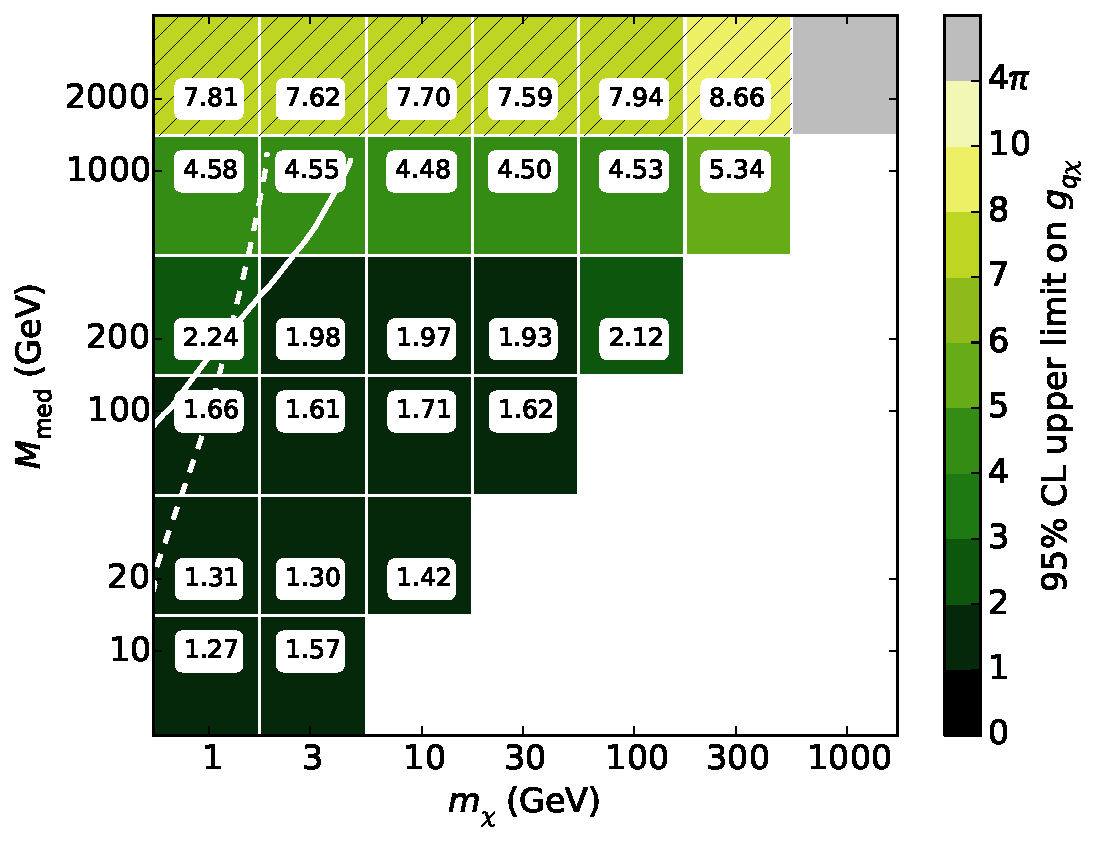
\includegraphics[width=0.6\textwidth]{figures/grid_allpoints_TSD_rat1.pdf}
    \caption{Upper limit on the coupling $\gqX$ for the tS model, in the \monoZ channel. The grey region represents the phase space where no meaningful limit was obtained. The hatched region represents a limit which leads to a width greater than $\Mmed / 2$, so the validity of the calculation begins to fail.}
    \label{fig:MonoZ_TSD_couplinglimit}
\end{figure}

Mono-Z limits discussion here. Overall uncertainty on $\sqrtgqgX$ generally $ < 10\%$, up to 80$\%$. Large DM masses: small cross sections, limited by ATLAS analysis optimisation, requires more data or further optimisation. Small DM masses: have low $\met$, would require more statistics.

\subsection{Mono-$W/Z$ channel}

\begin{figure}[h]
  \centering
    \begin{subfigure}[t]{0.495\textwidth}
      \centering
      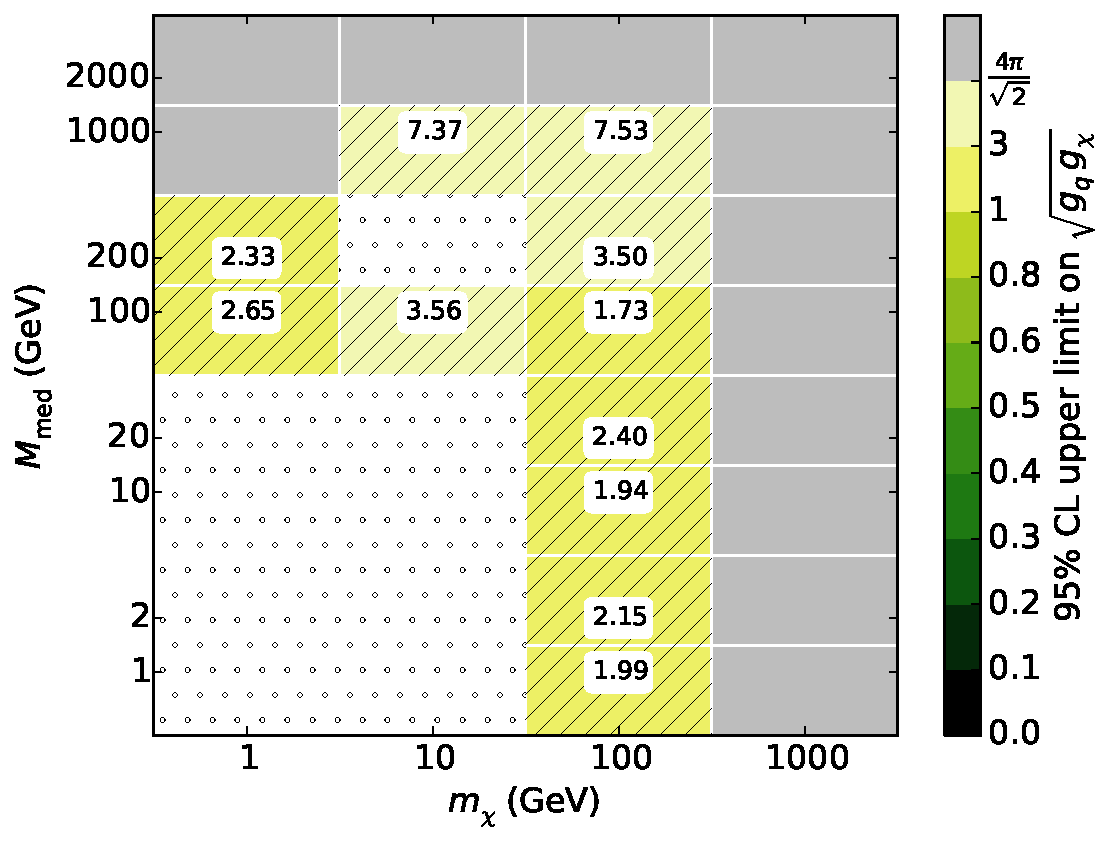
\includegraphics[width=1.\textwidth]{figures/grid_basepoints_SVD_rat05_monoWZ.pdf}
      \caption{}
    \end{subfigure}
    \begin{subfigure}[t]{0.495\textwidth}
      \centering
      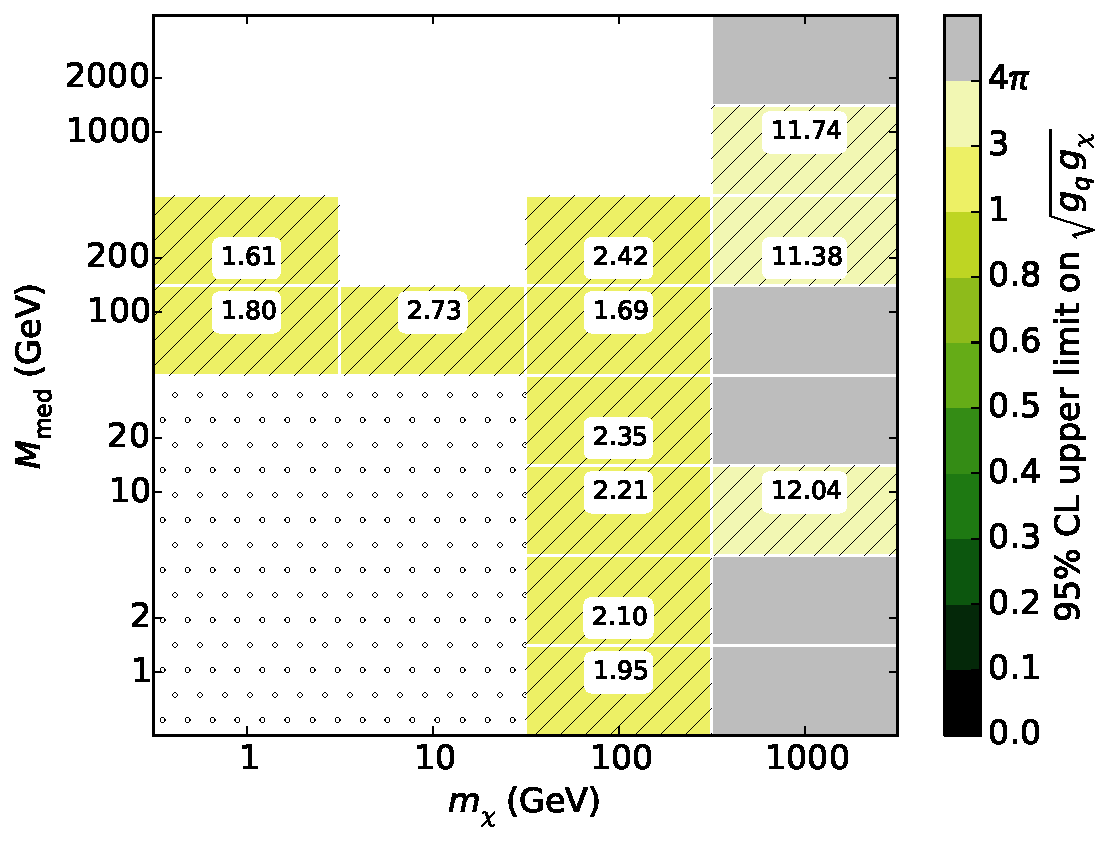
\includegraphics[width=1.\textwidth]{figures/grid_basepoints_SVD_rat1_monoWZ.pdf}
      \caption{}
    \end{subfigure}
    \begin{subfigure}[t]{0.495\textwidth}
      \centering
      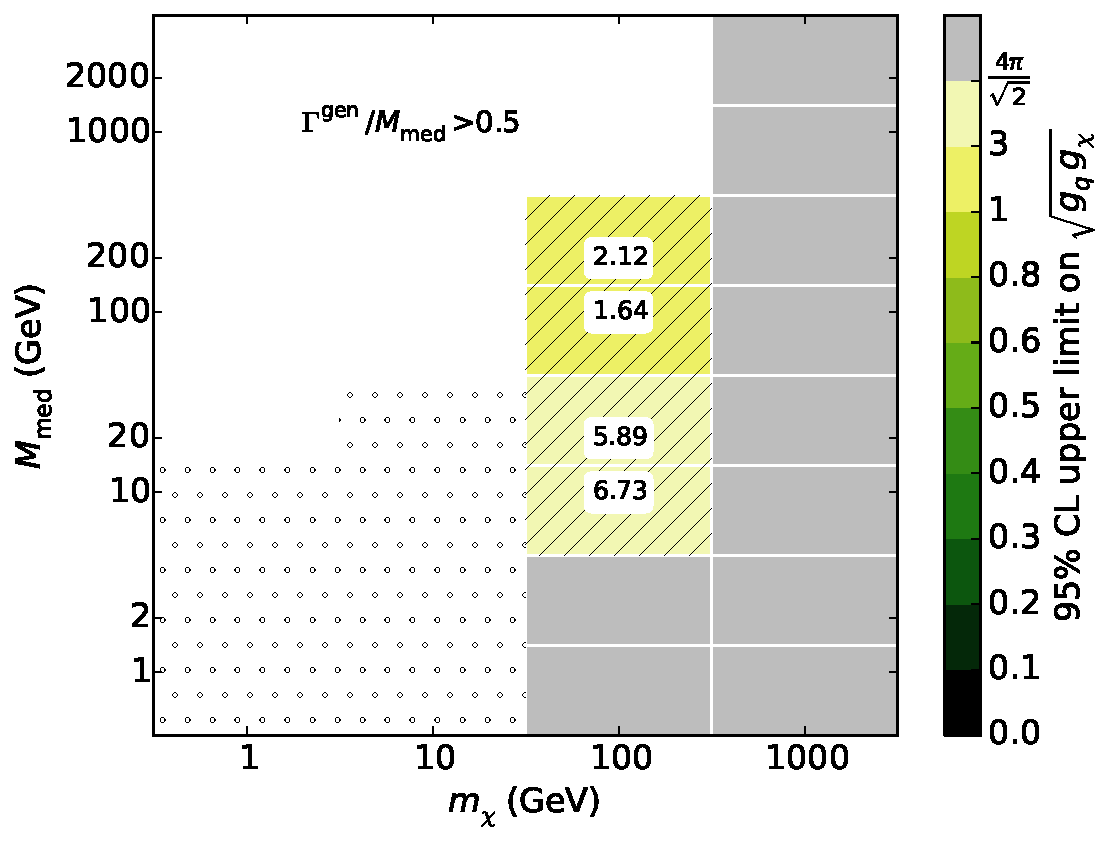
\includegraphics[width=1.\textwidth]{figures/grid_basepoints_SVD_rat2_monoWZ.pdf}
      \caption{}
    \end{subfigure}
    \begin{subfigure}[t]{0.495\textwidth}
      \centering
      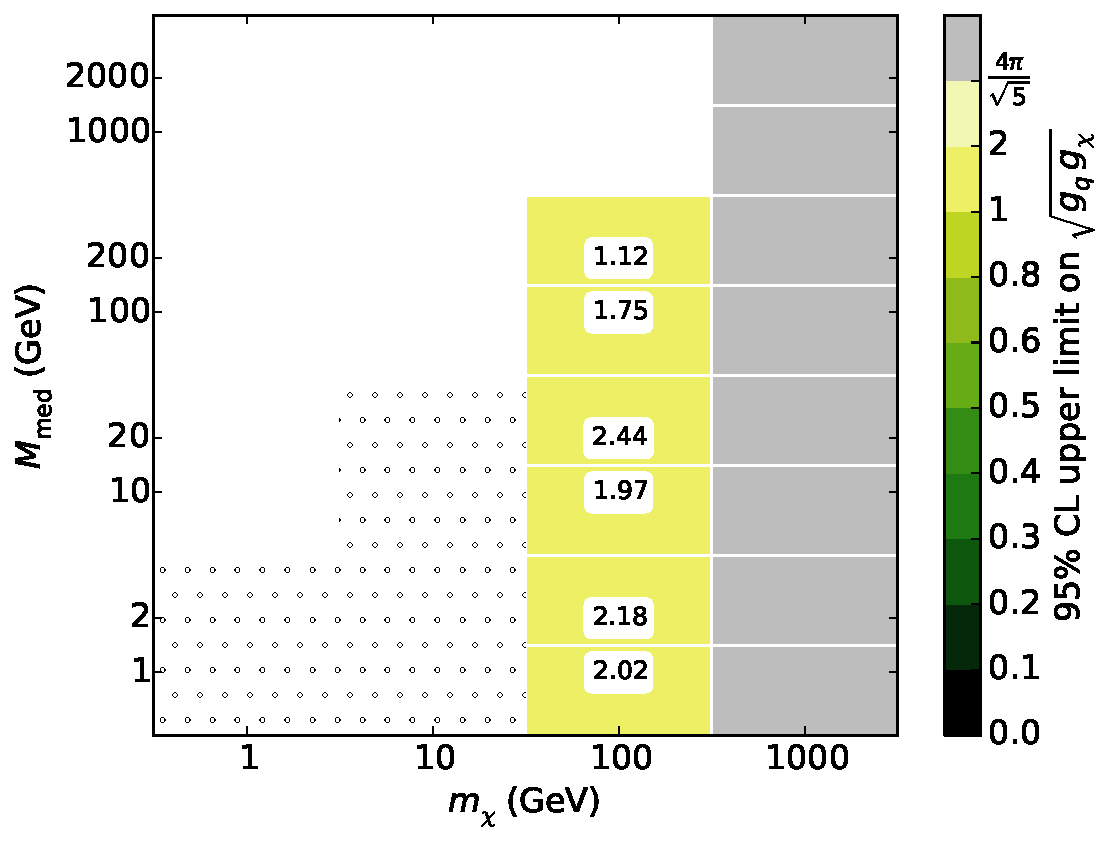
\includegraphics[width=1.\textwidth]{figures/grid_basepoints_SVD_rat5_monoWZ.pdf}
      \caption{}
    \end{subfigure}
    \caption{Upper limits on the coupling for the sV model, in the \monoWZ channel, for $\gX / \gq$ = 0.5 (a), 1 (b), 2 (c) and 5 (d). The grey region represents the phase space where no meaningful limit was obtained. The hatched region represents a limit which leads to a width greater than $\Mmed / 2$, so the validity of the calculation begins to fail.}
    \label{fig:MonoWZ_SVD_couplinglimit}
\end{figure}

\begin{figure}[h]
  \centering
    \begin{subfigure}[t]{0.495\textwidth}
      \centering
      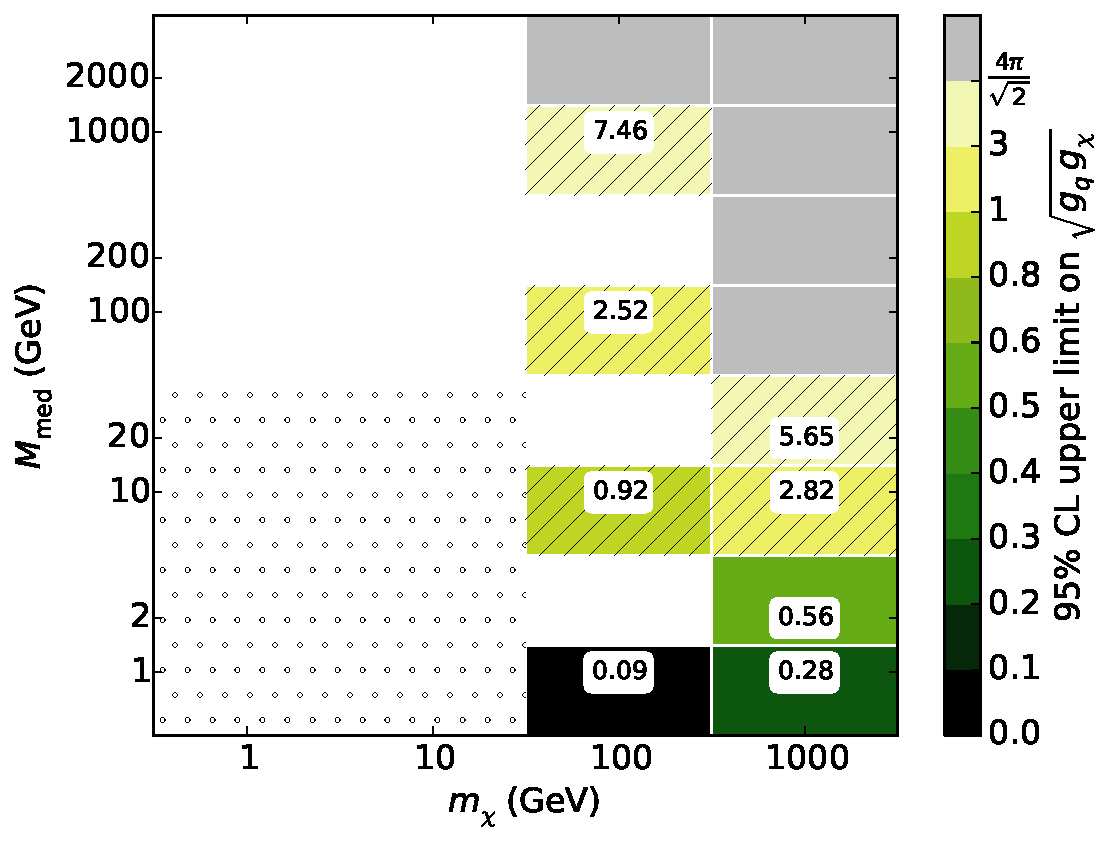
\includegraphics[width=1.\textwidth]{figures/grid_basepoints_SAD_rat05_monoWZ.pdf}
      \caption{}
    \end{subfigure}
    \begin{subfigure}[t]{0.495\textwidth}
      \centering
      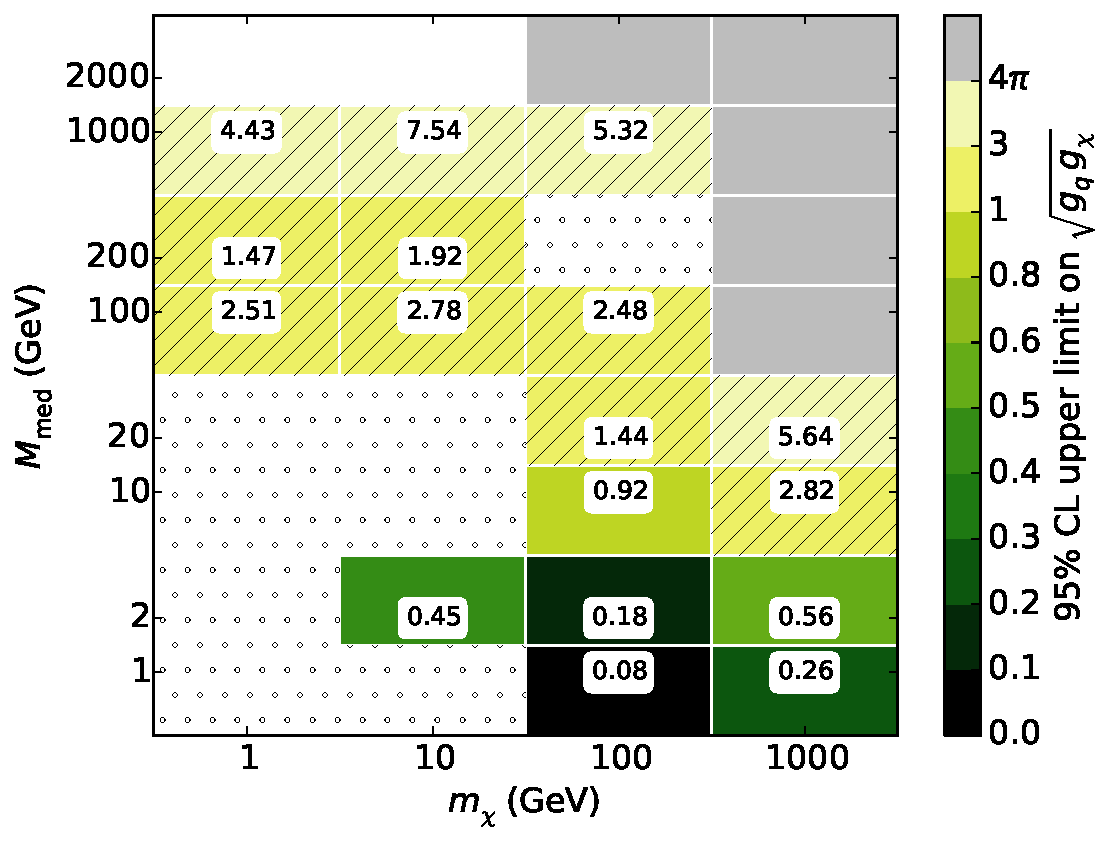
\includegraphics[width=1.\textwidth]{figures/grid_basepoints_SAD_rat1_monoWZ.pdf}
      \caption{}
    \end{subfigure}
    \begin{subfigure}[t]{0.495\textwidth}
      \centering
      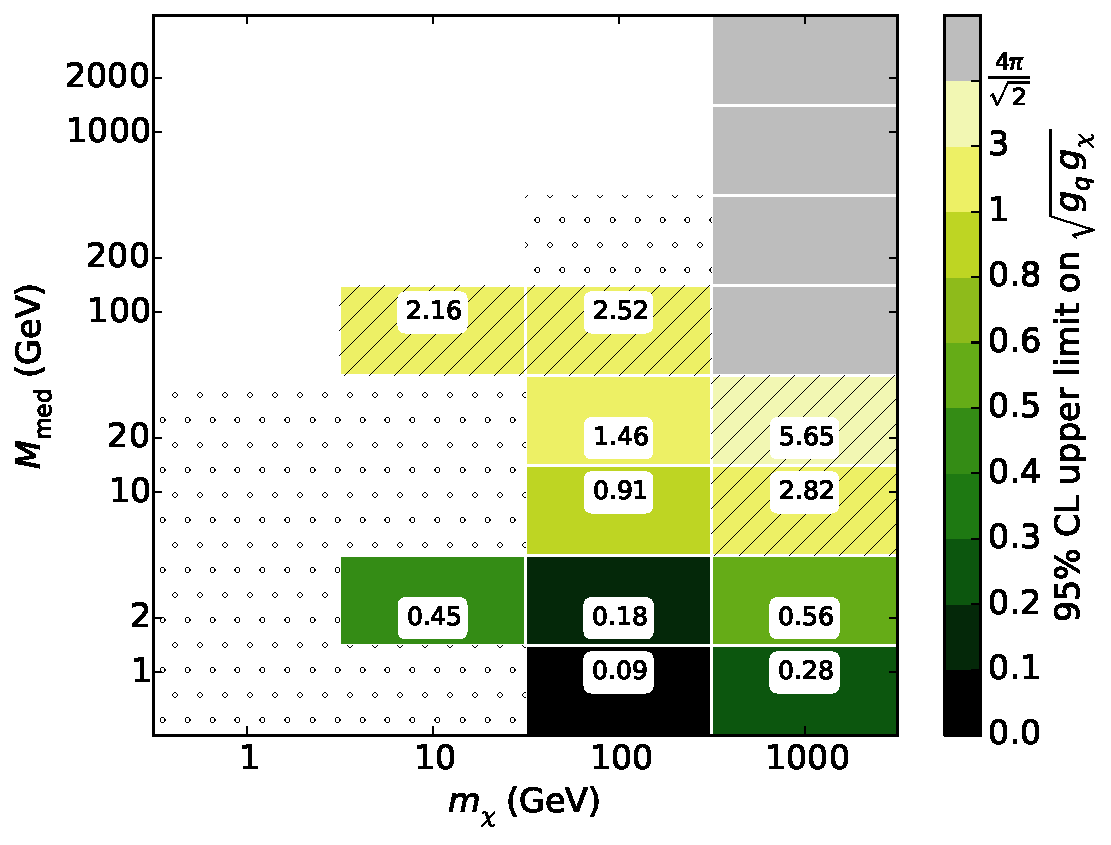
\includegraphics[width=1.\textwidth]{figures/grid_basepoints_SAD_rat2_monoWZ.pdf}
      \caption{}
    \end{subfigure}
    \begin{subfigure}[t]{0.495\textwidth}
      \centering
      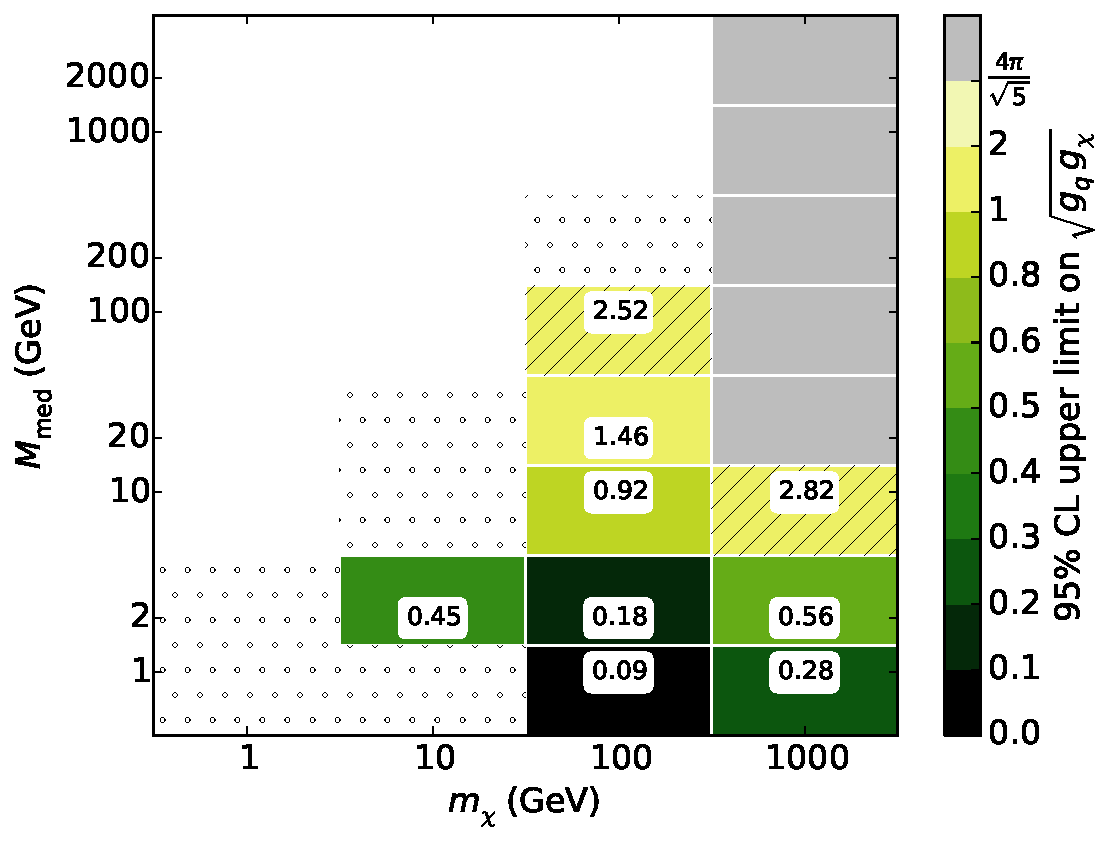
\includegraphics[width=1.\textwidth]{figures/grid_basepoints_SAD_rat5_monoWZ.pdf}
      \caption{}
    \end{subfigure}
    \caption{Upper limits on the coupling for the sA model, in the \monoWZ channel, for $\gX / \gq$ = 0.5 (a), 1 (b), 2 (c) and 5 (d). The grey region represents the phase space where no meaningful limit was obtained. The hatched region represents a limit which leads to a width greater than $\Mmed / 2$, so the validity of the calculation begins to fail.}
    \label{fig:MonoWZ_SAD_couplinglimit}
\end{figure}

\begin{figure}[!h]
  \centering
    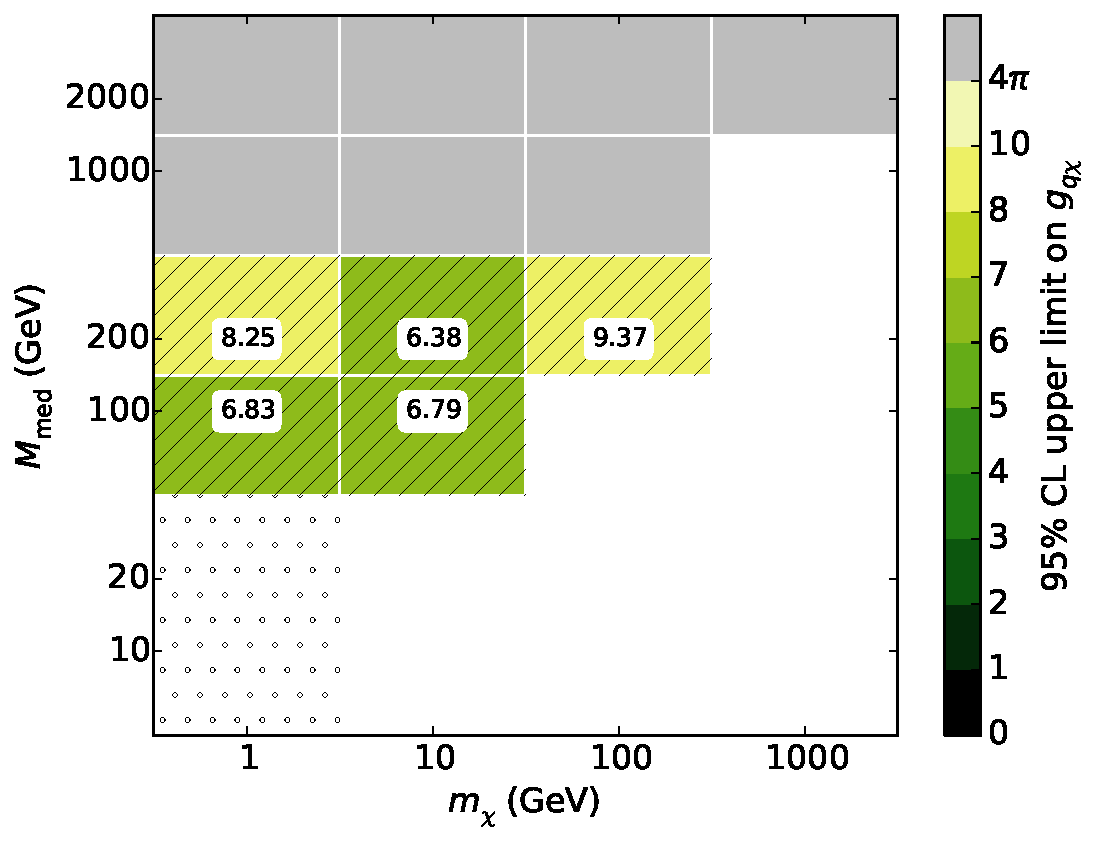
\includegraphics[width=0.6\textwidth]{figures/grid_basepoints_TSD_rat1_monoWZ.pdf}
    \caption{Upper limit on the coupling $\gqX$ for the tS model, in the \monoWZ channel. The grey region represents the phase space where no meaningful limit was obtained. The hatched region represents a limit which leads to a width greater than $\Mmed / 2$, so the validity of the calculation begins to fail.}
    \label{fig:MonoWZ_TSD_couplinglimit}
\end{figure}

Mono-W/Z limits discussion here.

\begin{figure}[h]
  \centering
    \begin{subfigure}[t]{0.325\textwidth}
      \centering
      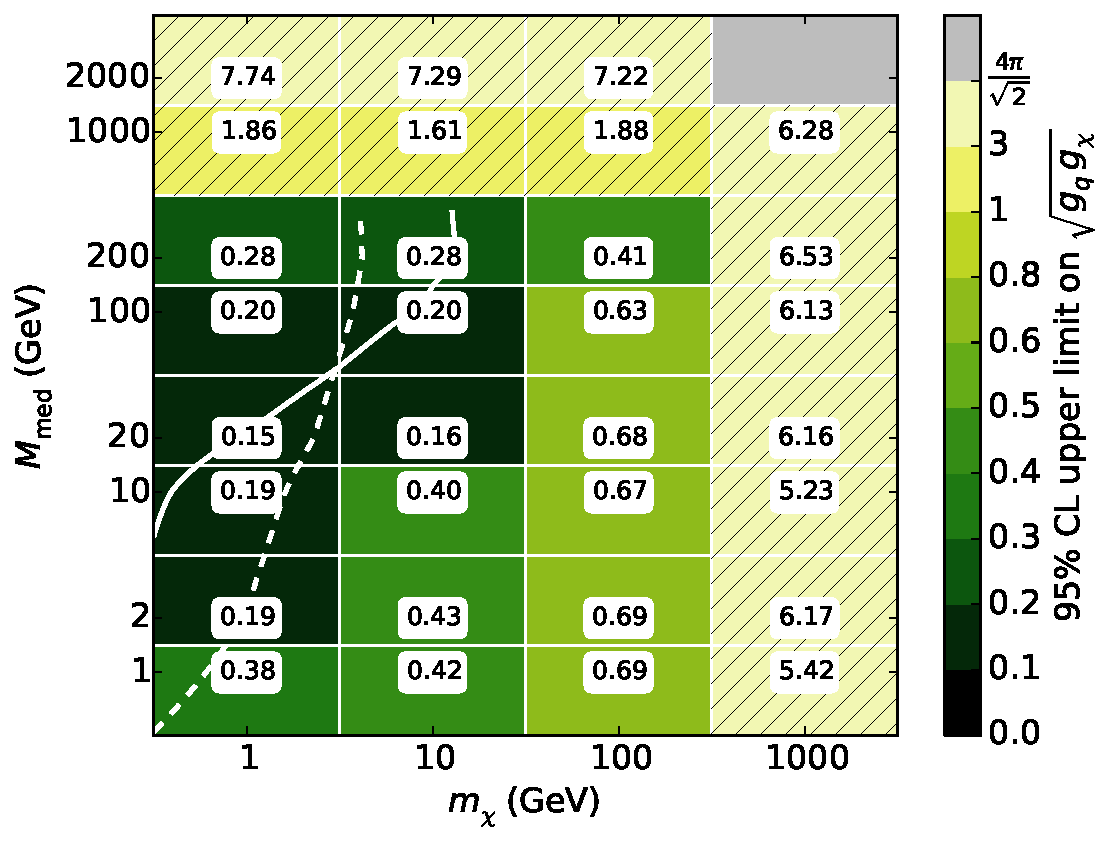
\includegraphics[width=1.\textwidth]{figures/grid_basepoints_SVD_rat05_monojet.pdf}
      \caption{}
    \end{subfigure}
    \begin{subfigure}[t]{0.325\textwidth}
      \centering
      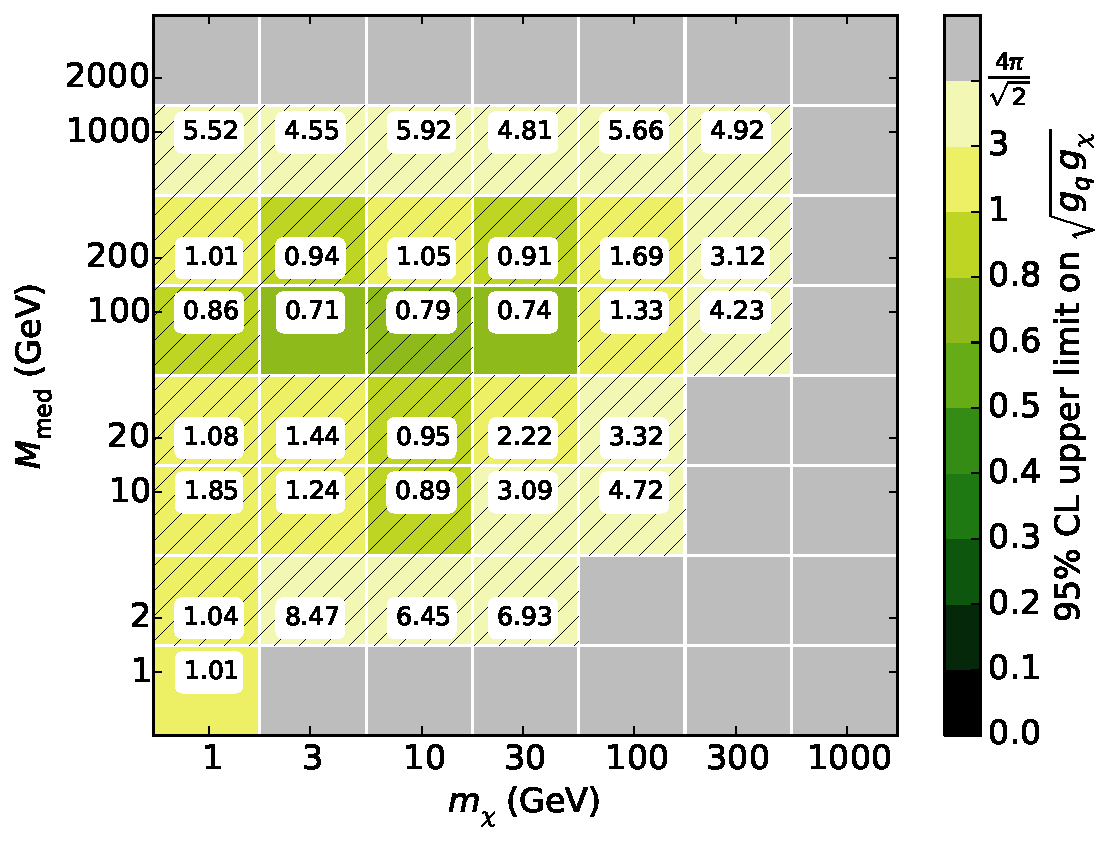
\includegraphics[width=1.\textwidth]{figures/grid_allpoints_SVD_rat05.pdf}
      \caption{}
    \end{subfigure}
    \begin{subfigure}[t]{0.325\textwidth}
      \centering
      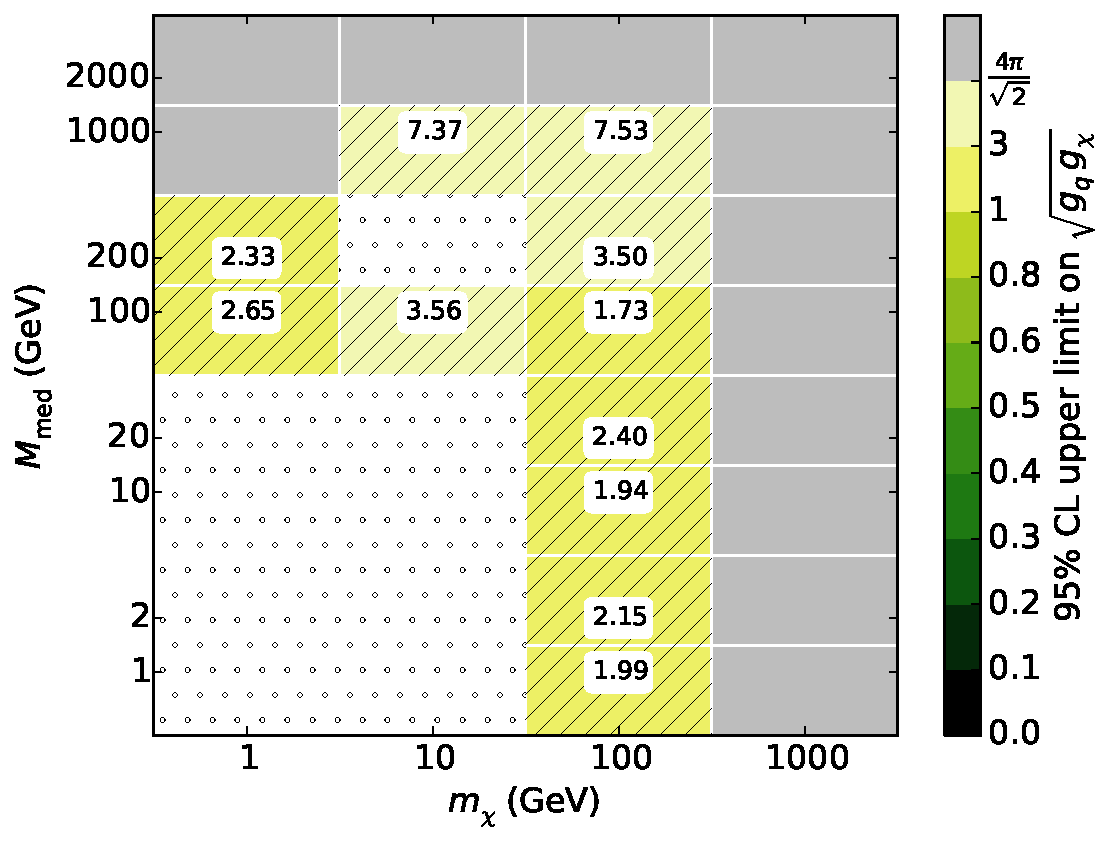
\includegraphics[width=1.\textwidth]{figures/grid_basepoints_SVD_rat05_monoWZ.pdf}
      \caption{}
    \end{subfigure}
    \begin{subfigure}[t]{0.325\textwidth}
      \centering
      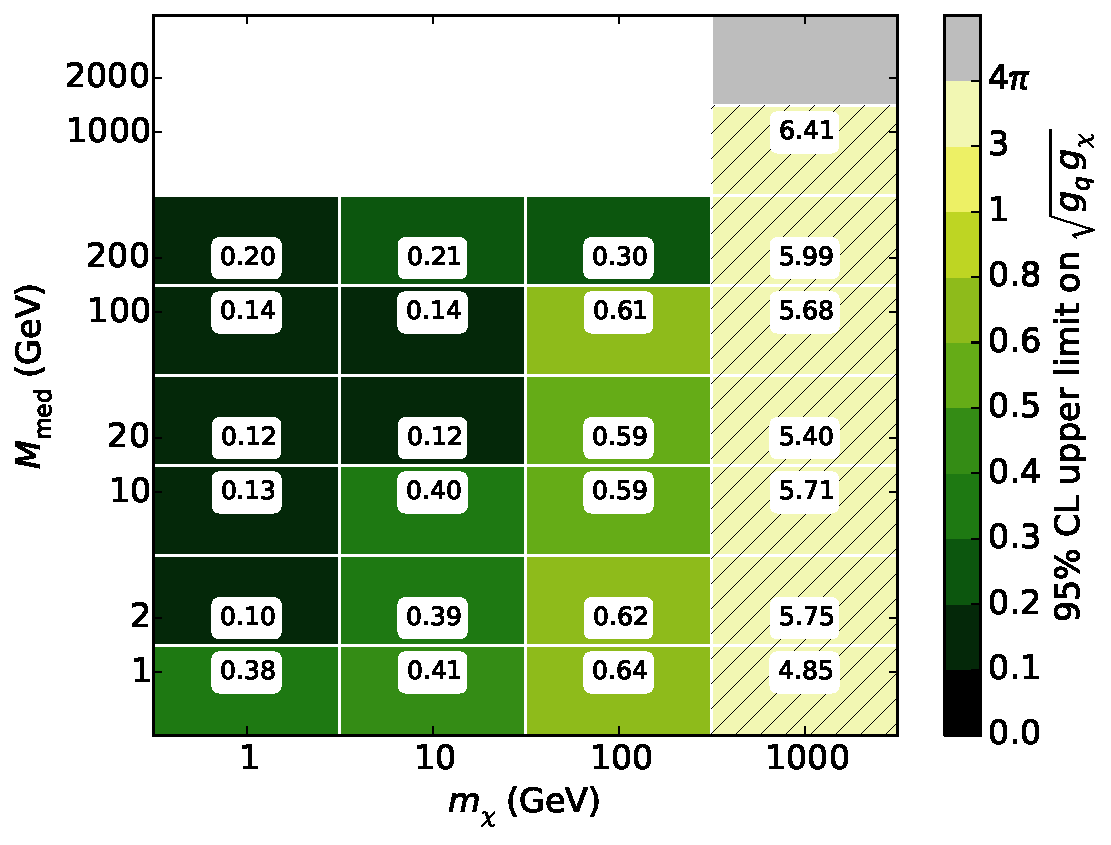
\includegraphics[width=1.\textwidth]{figures/grid_basepoints_SVD_rat1_monojet.pdf}
      \caption{}
    \end{subfigure}
    \begin{subfigure}[t]{0.325\textwidth}
      \centering
      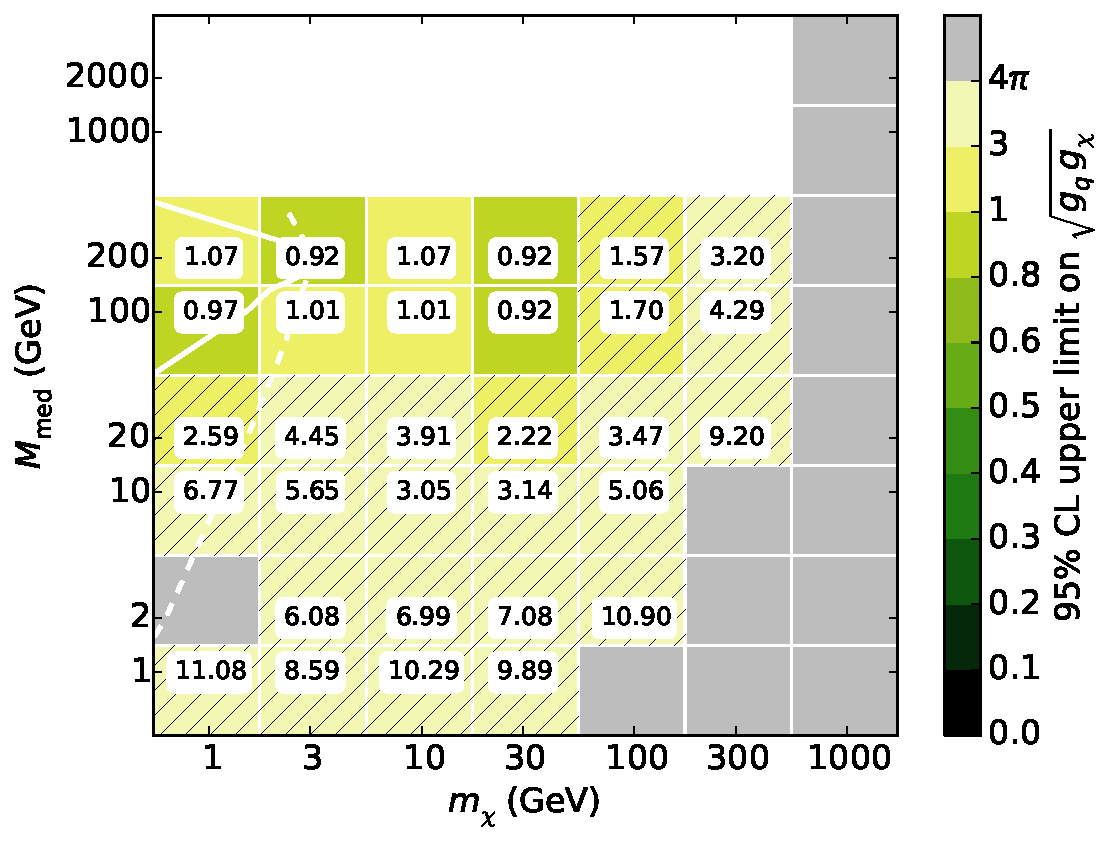
\includegraphics[width=1.\textwidth]{figures/grid_allpoints_SVD_rat1.pdf}
      \caption{}
    \end{subfigure}
    \begin{subfigure}[t]{0.325\textwidth}
      \centering
      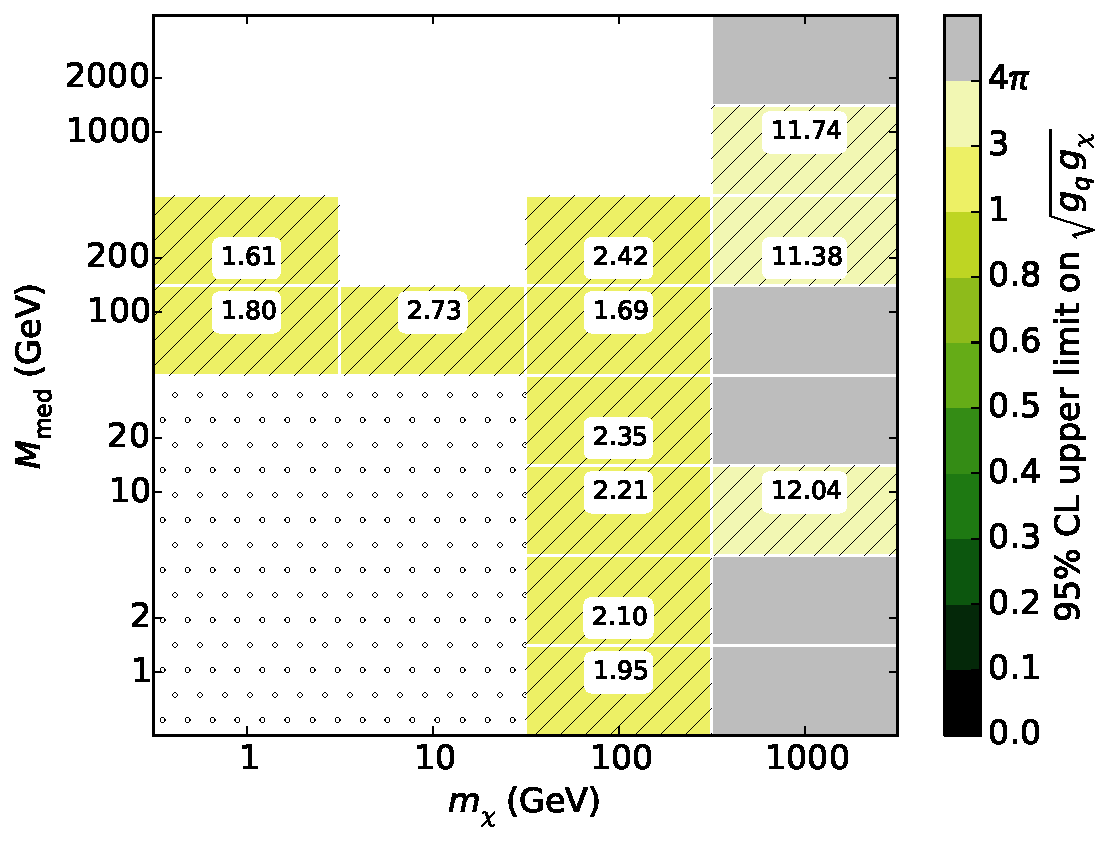
\includegraphics[width=1.\textwidth]{figures/grid_basepoints_SVD_rat1_monoWZ.pdf}
      \caption{}
    \end{subfigure}
    \begin{subfigure}[t]{0.325\textwidth}
      \centering
      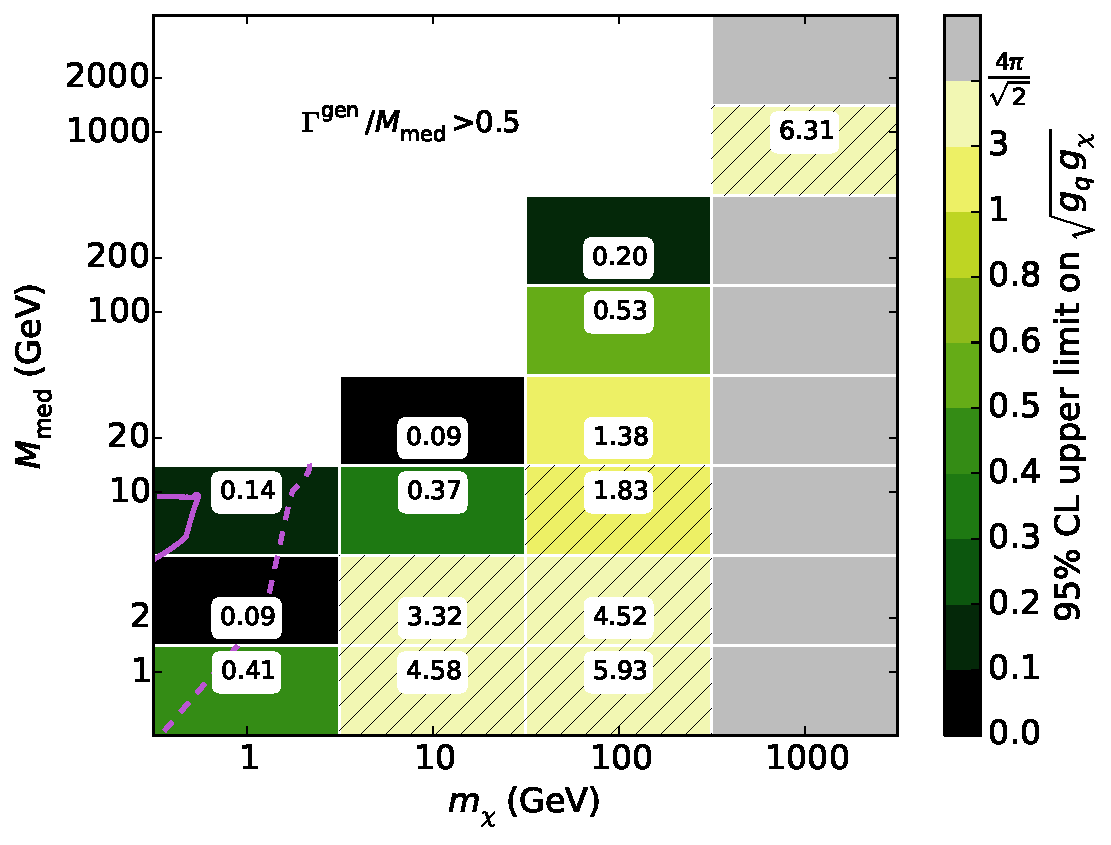
\includegraphics[width=1.\textwidth]{figures/grid_basepoints_SVD_rat2_monojet.pdf}
      \caption{}
    \end{subfigure}
    \begin{subfigure}[t]{0.325\textwidth}
      \centering
      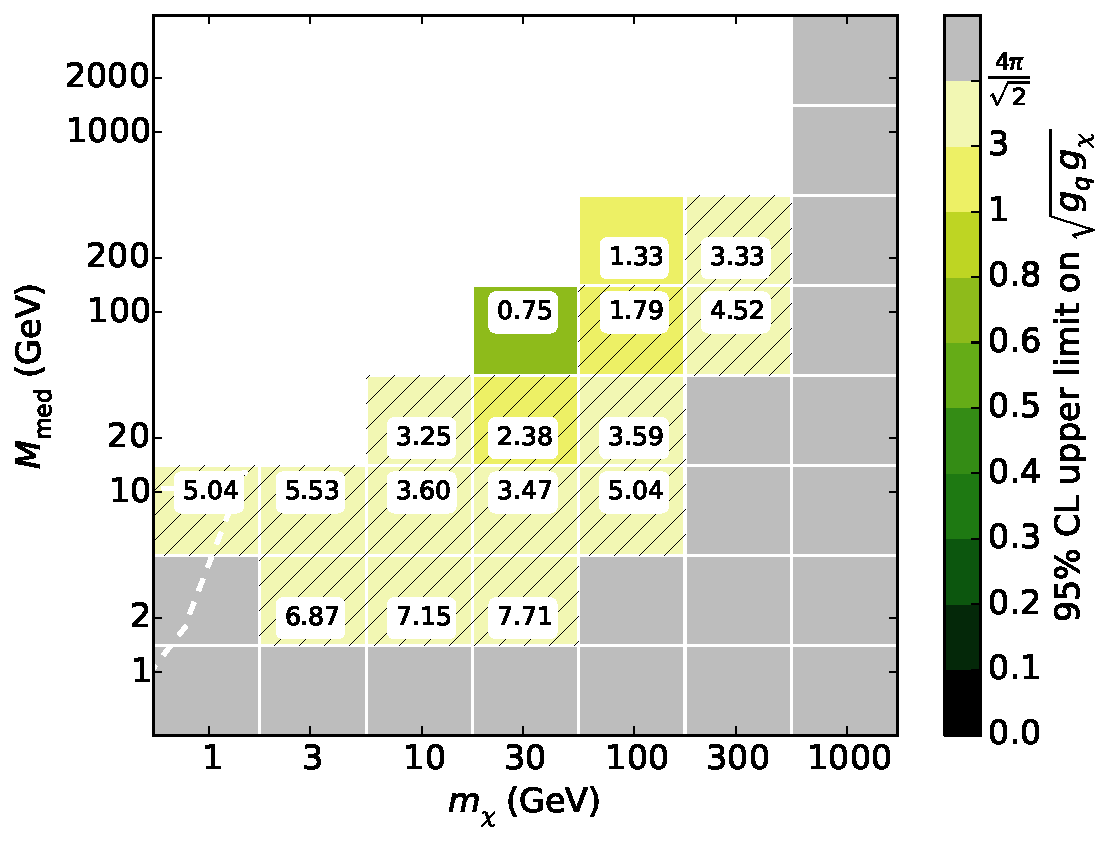
\includegraphics[width=1.\textwidth]{figures/grid_allpoints_SVD_rat2.pdf}
      \caption{}
    \end{subfigure}
    \begin{subfigure}[t]{0.325\textwidth}
      \centering
      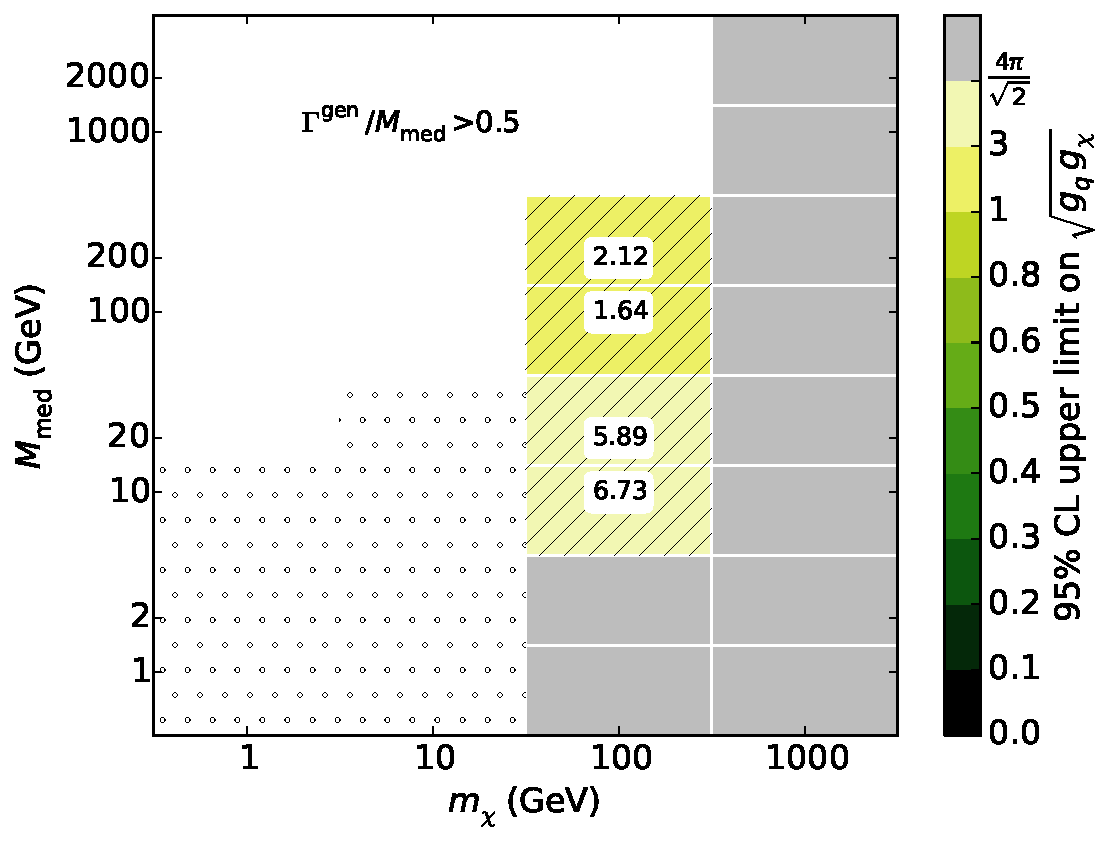
\includegraphics[width=1.\textwidth]{figures/grid_basepoints_SVD_rat2_monoWZ.pdf}
      \caption{}
    \end{subfigure}
    \begin{subfigure}[t]{0.325\textwidth}
      \centering
      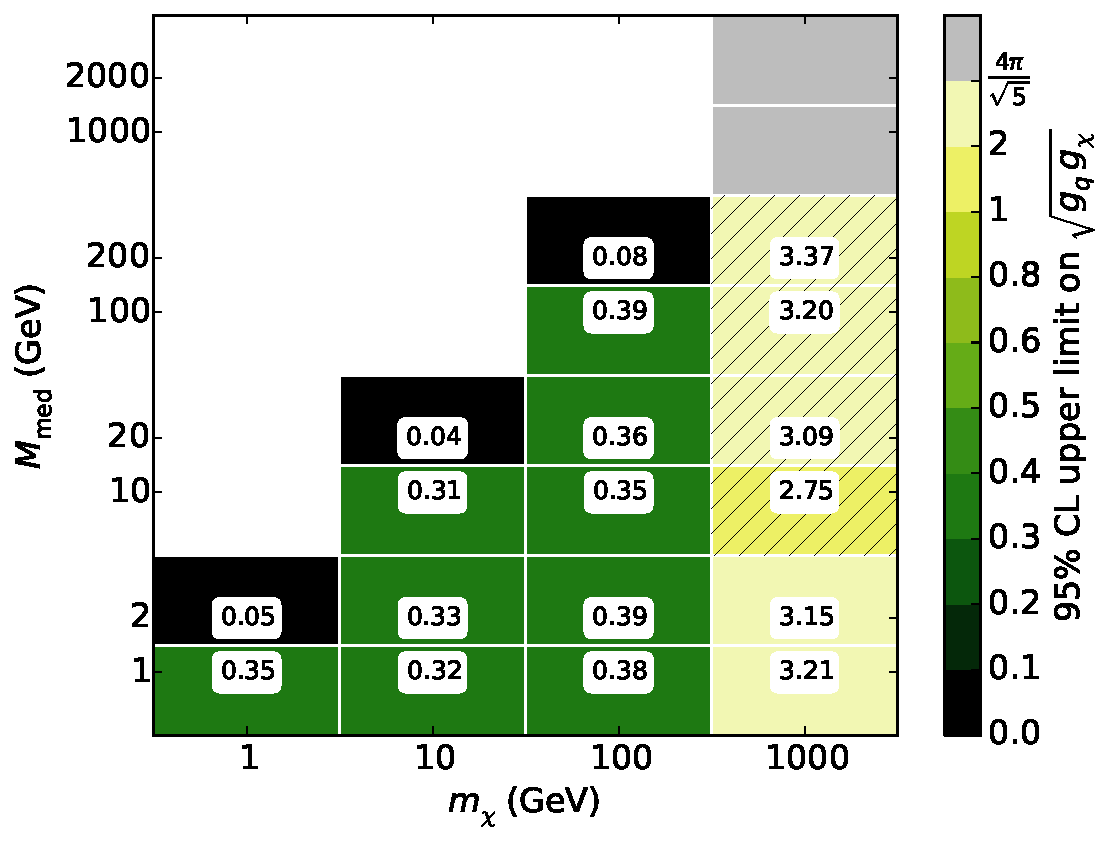
\includegraphics[width=1.\textwidth]{figures/grid_basepoints_SVD_rat5_monojet.pdf}
      \caption{}
    \end{subfigure}
    \begin{subfigure}[t]{0.325\textwidth}
      \centering
      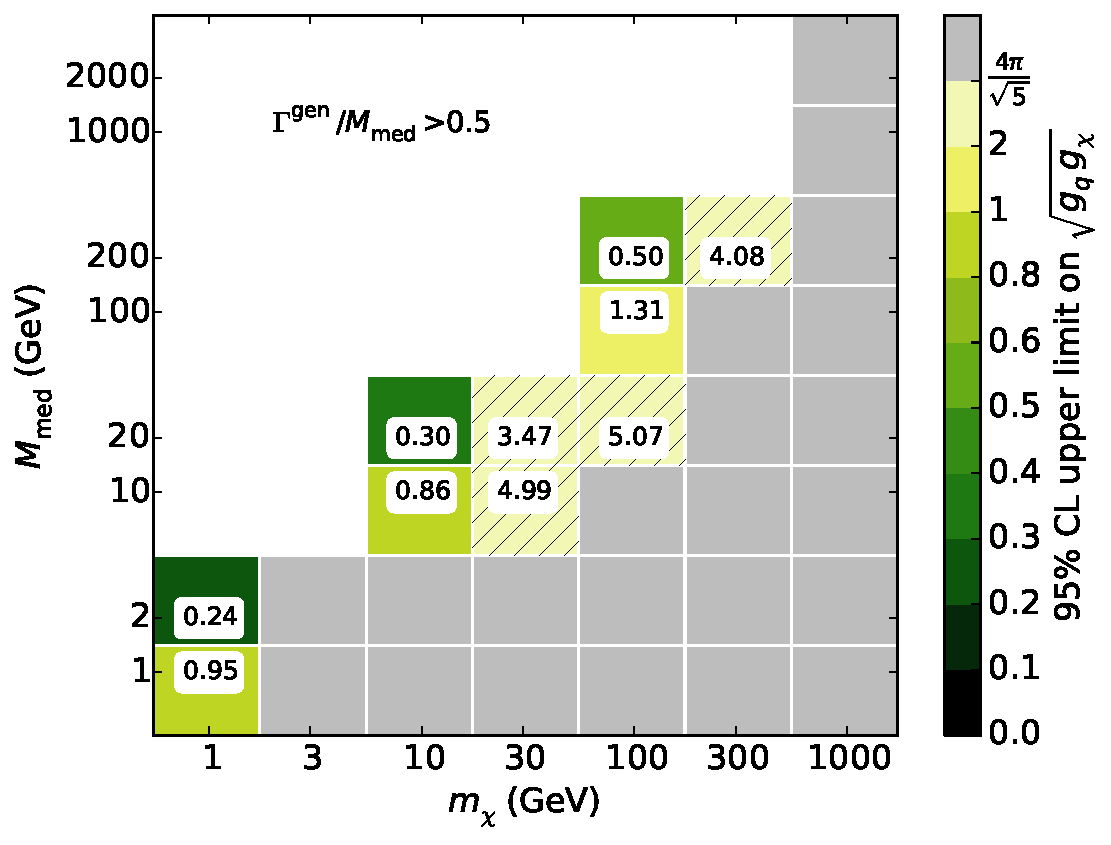
\includegraphics[width=1.\textwidth]{figures/grid_allpoints_SVD_rat5.pdf}
      \caption{}
    \end{subfigure}
    \begin{subfigure}[t]{0.325\textwidth}
      \centering
      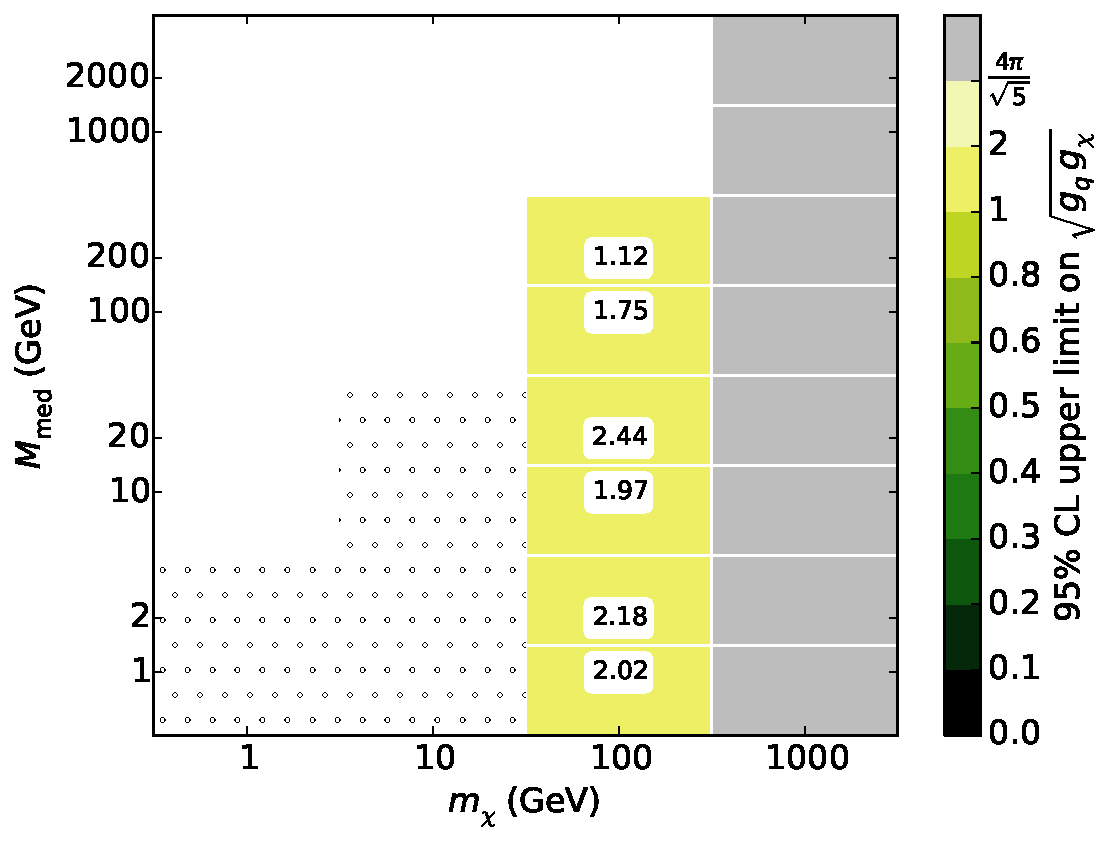
\includegraphics[width=1.\textwidth]{figures/grid_basepoints_SVD_rat5_monoWZ.pdf}
      \caption{}
    \end{subfigure}
    \caption{Testing 12 on a page. Upper limits on the coupling for the sV model, in the \monojet (left), \monoZ (centre) and \monoWZ (right) channels, for $\gX / \gq$ = 0.5, 1, 2 and 5 (top to bottom). The grey region represents the phase space where no meaningful limit was obtained. The hatched region represents a limit which leads to a width greater than $\Mmed / 2$, so the validity of the calculation begins to fail. The dotted region represents phase space where insufficient statistics were available.}
\end{figure}

\begin{figure}[h]
  \centering
    \begin{subfigure}[t]{0.495\textwidth}
      \centering
      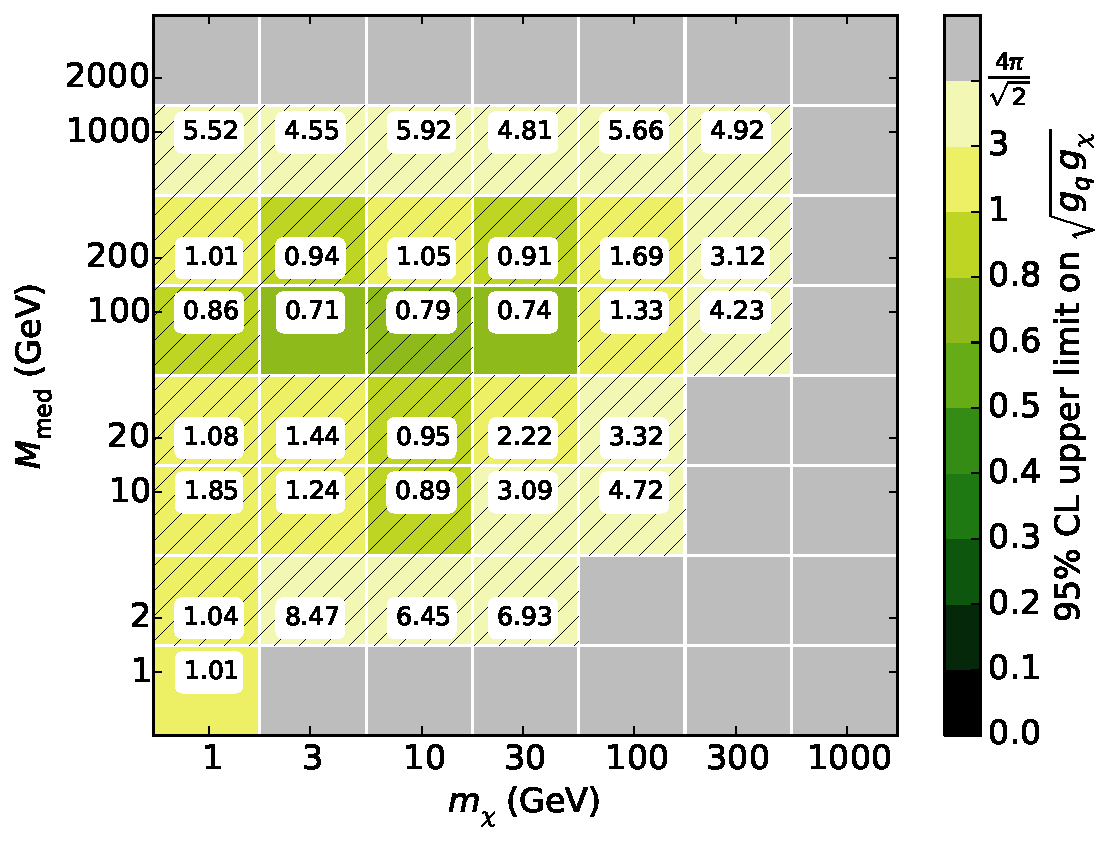
\includegraphics[width=1.\textwidth]{figures/grid_allpoints_SVD_rat05.pdf}
    \end{subfigure}
    \begin{subfigure}[t]{0.495\textwidth}
      \centering
      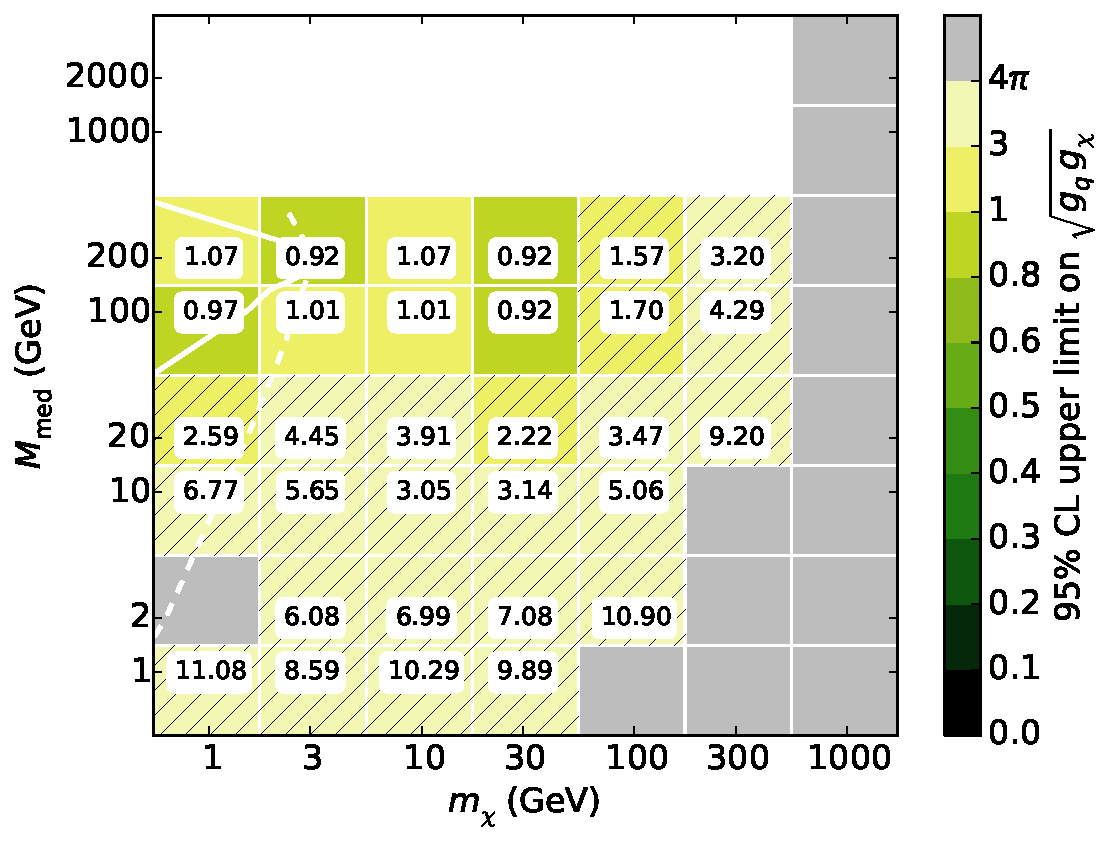
\includegraphics[width=1.\textwidth]{figures/grid_allpoints_SVD_rat1.pdf}
    \end{subfigure}
    \begin{subfigure}[t]{0.495\textwidth}
      \centering
      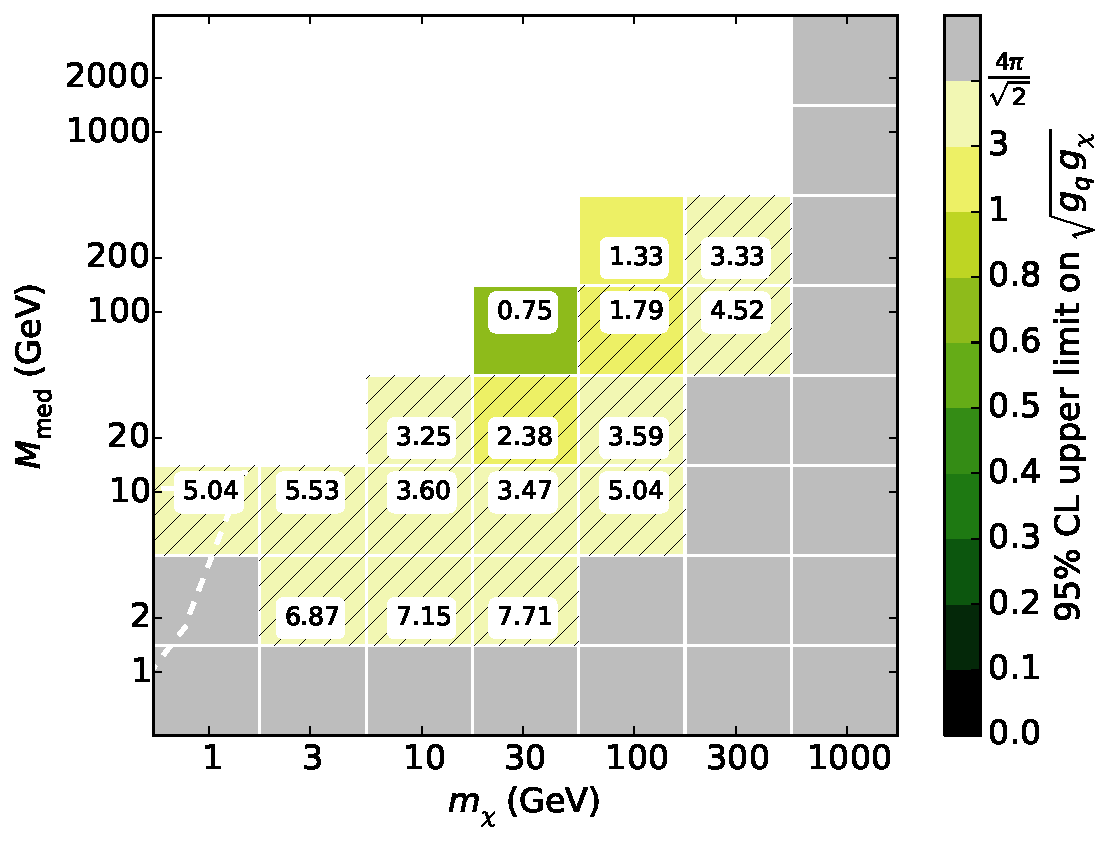
\includegraphics[width=1.\textwidth]{figures/grid_allpoints_SVD_rat2.pdf}
    \end{subfigure}
    \begin{subfigure}[t]{0.495\textwidth}
      \centering
      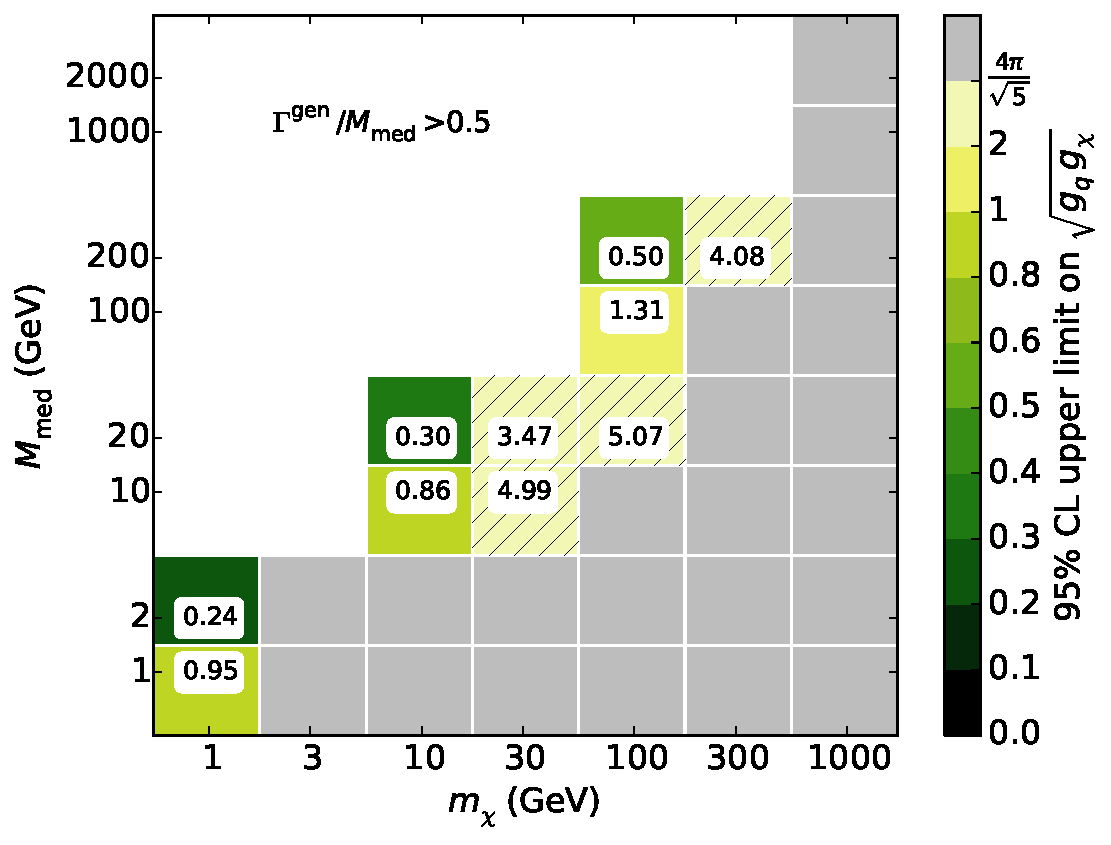
\includegraphics[width=1.\textwidth]{figures/grid_allpoints_SVD_rat5.pdf}
    \end{subfigure}
    \begin{subfigure}[t]{0.495\textwidth}
      \centering
      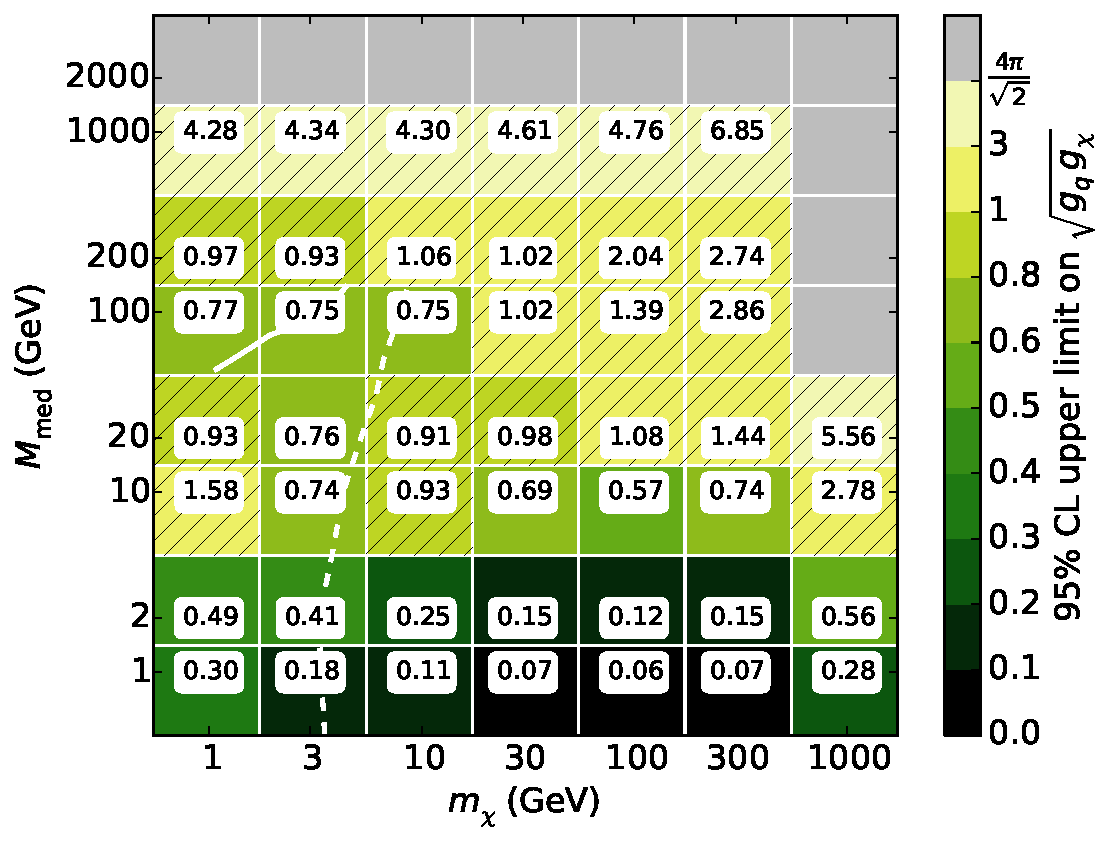
\includegraphics[width=1.\textwidth]{figures/grid_allpoints_SAD_rat05.pdf}
    \end{subfigure}
    \begin{subfigure}[t]{0.495\textwidth}
      \centering
      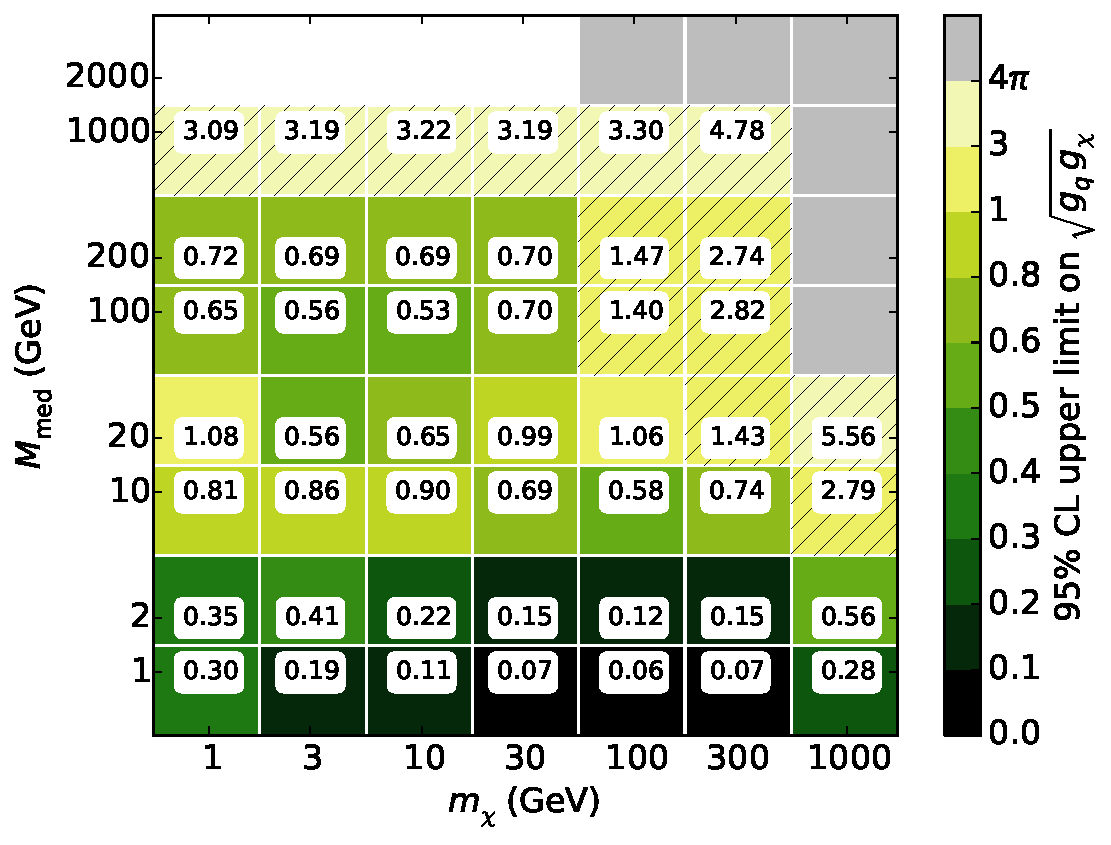
\includegraphics[width=1.\textwidth]{figures/grid_allpoints_SAD_rat1.pdf}
    \end{subfigure}
    \begin{subfigure}[t]{0.495\textwidth}
      \centering
      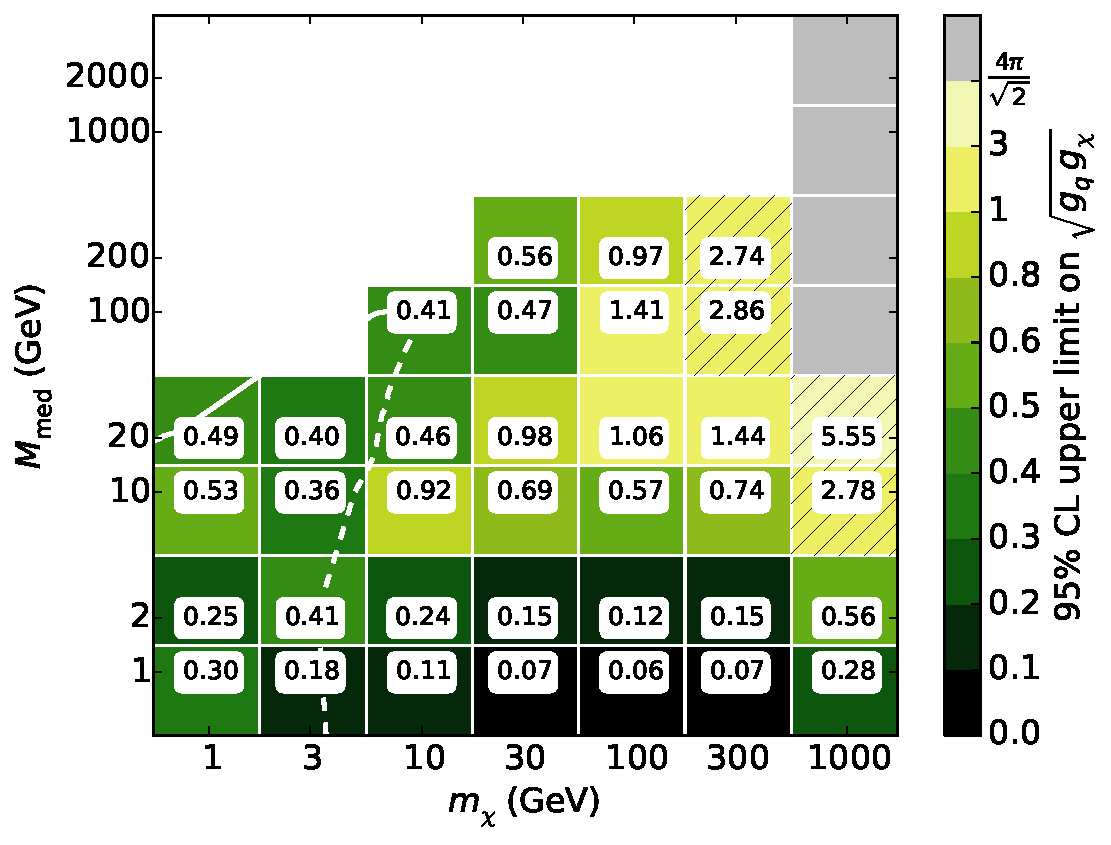
\includegraphics[width=1.\textwidth]{figures/grid_allpoints_SAD_rat2.pdf}
    \end{subfigure}
    \begin{subfigure}[t]{0.495\textwidth}
      \centering
      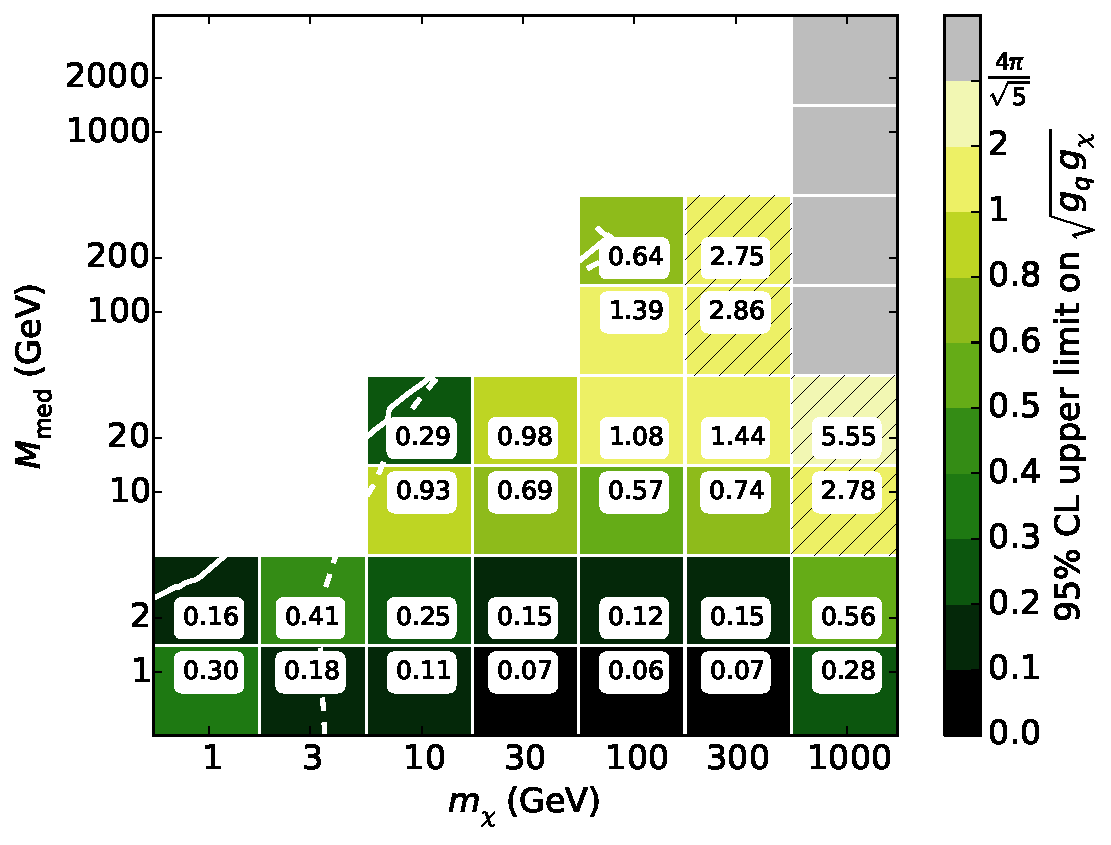
\includegraphics[width=1.\textwidth]{figures/grid_allpoints_SAD_rat5.pdf}
    \end{subfigure}
    \caption{Testing 8 on a page without captions. Upper limits on the coupling for the sV (top two rows) and sA (bottom two rows) models in the \monoZ channel, for $\gX / \gq$ = 0.5, 1, 2 and 5. The grey region represents the phase space where no meaningful limit was obtained. The hatched region represents a limit which leads to a width greater than $\Mmed / 2$, so the validity of the calculation begins to fail. The dotted region represents phase space where insufficient statistics were available.}
\end{figure}
